\documentclass[12pt,openany]{book}
% Public edition switches.
\newif\ifpublicmanual
\newif\ifinternalmanual
\publicmanualtrue
\internalmanualfalse
\newcommand{\ManualEdition}{Public User Manual}
\newcommand{\ManualAudience}{Public Users}

% Descriptive metadata only; title-page graphics are set in frontmatter/titlepage.tex.
\newcommand{\manualversion}{2.0}

\usepackage[a4paper,scale=0.8,centering]{geometry}
\usepackage{fancyhdr}
\usepackage{setspace}
\usepackage{titlesec}
\usepackage{tocloft}
\usepackage{hyperref}
\usepackage{graphicx}
\graphicspath{{assets/}}
\usepackage{xcolor}
\usepackage{amsmath}
\usepackage{enumitem}
\usepackage{hyperref}
\usepackage{caption}
\usepackage{setspace}
\usepackage{helvet}
\usepackage{times}
\usepackage[backend=biber,sorting=none]{biblatex}
\usepackage{indentfirst}
\usepackage{listings}
\usepackage{lipsum}
\usepackage{accsupp}
\usepackage{colortbl}
\usepackage{tabularx}
\usepackage{longtable}
\usepackage{xltabular}
\usepackage{ltablex}

\addbibresource[location=local]{references-build.bib}


%!!!!!!!!! Temporary Use !!!!!!!!!!!!!!!!!!!!!!!!!!
%!!!!!!!!! Temporary Use !!!!!!!!!!!!!!!!!!!!!!!!!!


\definecolor{backgray}{rgb}{0.92,0.92,0.92}
\definecolor{mygray}{rgb}{0.5,0.5,0.5}
\definecolor{mygreen}{rgb}{0,0.6,0}
\definecolor{myorange}{rgb}{1.0,0.4,0}
\definecolor{myredstring}{rgb}{0.76,0.06,0.15}

%%%%%%%%%%%%%%%%%%%%%%%%%%%%%%%%%%%%%%%%%%%%%%%%%%%%%%%%%%%%%%%%%%%%%%%%%%%%%%%%
% Shell script definition
%%%%%%%%%%%%%%%%%%%%%%%%%%%%%%%%%%%%%%%%%%%%%%%%%%%%%%%%%%%%%%%%%%%%%%%%%%%%%%%%
\lstnewenvironment{lst-installation}{
  \lstset{
  backgroundcolor=\color{backgray},
  commentstyle=\color{mygreen},
  keywordstyle=\color{magenta},
  numberstyle=\tiny\color{mygray},
  stringstyle=\color{myredstring},
  basicstyle=\ttfamily\small,
  %basicstyle=\ttfamily\fontsize{10pt}{10pt}\selectfont,
  breakatwhitespace=false,
  breaklines=true,
  captionpos=b,
  keepspaces=true,
  numbers=none,
  numbersep=5pt,
  showspaces=false,
  showstringspaces=false,
  showtabs=false,
  tabsize=2,
  escapechar=@
  }
}{}

%%%%%%%%%%%%%%%%%%%%%%%%%%%%%%%%%%%%%%%%%%%%%%%%%%%%%%%%%%%%%%%%%%%%%%%%%%%%%%%%
% Script block definition
%%%%%%%%%%%%%%%%%%%%%%%%%%%%%%%%%%%%%%%%%%%%%%%%%%%%%%%%%%%%%%%%%%%%%%%%%%%%%%%%
\definecolor{scriptcapgray}{rgb}{0.3,0.3,0.3}

\newcounter{scriptnum}[chapter]

\newcommand{\scriptnum}[1]{\noindent\#\hspace{6.73cm}
  \refstepcounter{scriptnum}
  \hypertarget{#1}{
  \textcolor{scriptcapgray}
  {\textbf{\textrm{ Script \thechapter-\arabic{scriptnum}}}}}\label{#1}}

\newcommand{\script}[2]{%
  \textcolor{blue}{\hyperlink{#2}{Script \ref{#1}-\ref{#2}}}%
}

\newcounter{examplenum}[chapter]

\newcommand{\examplenum}[1]{\noindent\#\hspace{6.65cm}
  \refstepcounter{examplenum}
  \hypertarget{#1}{
  \textcolor{scriptcapgray}
  {\textbf{\textrm{ Example \thechapter-\arabic{examplenum}}}}}\label{#1}}

\newcommand{\example}[2]{%
  \textcolor{blue}{\hyperlink{#2}{Example \ref{#1}-\ref{#2}}}%
}

\lstdefinelanguage{script}{
  morekeywords={\$,\$\$,\$\$\$,\$\$\$\$,\$\$\$\$\$},
  morecomment=[l]{\#},
  morestring=[b]", 
  alsoletter={-},
  morekeywords=[2]{postorb,postwfn,diabat-fphd,diabat-gmh,diabat-fcd,diabat-fed,diabat-fedfcd,diabat-utils-phasefix,statepack,stateset,mopack,statepack-ref,statepack-target,statepack-1,statepack-2,statepack-3},
}

\lstnewenvironment{lst-script}[1][]{
  \lstset{
  backgroundcolor=\color{backgray},
  commentstyle=\color{mygreen},
  keywordstyle=\color{blue},
  keywordstyle=[2]\color{magenta},
  numberstyle=\tiny\color{mygray},
  stringstyle=\color{myredstring},
  breakatwhitespace=false,
  breaklines=true,
  keepspaces=true,
  numbers=none,
  numbersep=5pt,
  showspaces=false,
  showstringspaces=false,
  showtabs=false,
  tabsize=2,
  basicstyle=\ttfamily\fontsize{10pt}{10pt}\selectfont,
  language=script,
  moredelim=[is][\color{magenta}]{<}{>},
  literate={\$}{{{\color{blue}\$}}}1 {~}{{{$\sim$}}}2,
  escapechar=@
  %aboveskip=1.5ex,
  %belowskip=-4ex
  %\textasciitilde
  }
}{}



%%%%%%%%%%%%%%%%%%%%%%%%%%%%%%%%%%%%%%%%%%%%%%%%%%%%%%%%%%%%%%%%%%%%%%%%%%%%%%%%
% Compatibility aliases for future source cleanup. These do not affect current
% output unless authors choose to use them in new chapters.
%%%%%%%%%%%%%%%%%%%%%%%%%%%%%%%%%%%%%%%%%%%%%%%%%%%%%%%%%%%%%%%%%%%%%%%%%%%%%%%%
\lstnewenvironment{ShellBlock}{\lstset{
  backgroundcolor=\color{backgray}, commentstyle=\color{mygreen}, keywordstyle=\color{magenta},
  numberstyle=\tiny\color{mygray}, stringstyle=\color{myredstring}, basicstyle=\ttfamily\small,
  breakatwhitespace=false, breaklines=true, captionpos=b, keepspaces=true, numbers=none,
  numbersep=5pt, showspaces=false, showstringspaces=false, showtabs=false, tabsize=2, escapechar=@
}}{}
\lstnewenvironment{DiabatScript}[1][]{\lstset{
  backgroundcolor=\color{backgray}, commentstyle=\color{mygreen}, keywordstyle=\color{blue},
  numberstyle=\tiny\color{mygray}, stringstyle=\color{myredstring}, breakatwhitespace=false,
  breaklines=true, keepspaces=true, numbers=none, numbersep=5pt, showspaces=false,
  showstringspaces=false, showtabs=false, tabsize=2,
  basicstyle=\ttfamily\fontsize{10pt}{10pt}\selectfont, language=script,
  moredelim=[is][\color{magenta}]{<}{>}, literate={\$}{{{\color{blue}\$}}}1 {~}{{{$\sim$}}}2, escapechar=@
}}{}

% File listings use the exact same visual parameters as the original lst-script blocks.
\lstdefinestyle{diabatfile}{
  backgroundcolor=\color{backgray},commentstyle=\color{mygreen},
  keywordstyle=\color{blue},keywordstyle=[2]\color{magenta},
  stringstyle=\color{myredstring},basicstyle=\ttfamily\fontsize{10pt}{10pt}\selectfont,
  breakatwhitespace=false,breaklines=true,keepspaces=true,numbers=none,
  showspaces=false,showstringspaces=false,showtabs=false,tabsize=2,
  language=script,moredelim=[is][\color{magenta}]{<}{>},escapechar=@,
  literate={\$}{{{\color{blue}\$}}}1
}
\lstdefinestyle{technicalfile}{
  backgroundcolor=\color{backgray},commentstyle=\color{mygreen},
  stringstyle=\color{myredstring},basicstyle=\ttfamily\fontsize{10pt}{10pt}\selectfont,
  breaklines=true,keepspaces=true,numbers=none,showstringspaces=false,
  morecomment=[l]{\#},morestring=[b]"
}

%%%%%%%%%%%%%%%%%%%%%%%%%%%%%%%%%%%%%%%%%%%%%%%%%%%%%%%%%%%%%%%%%%%%%%%%%%%%%%%%
% program name style
\newcommand{\prognameplain}{Diabat}

\newcommand{\proglinewidth}{0.5pt}

\newcommand{\progchar}[2]{%
  \begingroup
  \colorlet{progfill}{white!#2!black}%
  \pdfrender{
    TextRenderingMode=FillStroke,
    LineWidth=\proglinewidth,
    FillColor=progfill,
    StrokeColor=black
  }{#1}%
  \endgroup
}

\DeclareRobustCommand{\progname}{%
  \scalebox{0.85}{%
    {\fontfamily{qcs}\fontseries{m}\selectfont
      \progchar{D}{50}%
      i%
      a%
      \progchar{b}{50}%
      a%
      \progchar{t}{50}%
    }%
  }%
}

\newcommand{\exec}{\texttt{diabat}}
\newcommand{\Sec}[1]{Sec.\,\ref{#1}}

\newcommand{\manualnote}[1]{%
  {#1}%
}

% key text to emphasize
\definecolor{keyemphgray}{gray}{0.25}
\newcommand{\keyemph}[1]{%
  \textcolor{keyemphgray}{\emph{#1}}%
}

%%%%%%%%%%%%%%%%%%%%%%%%%%%%%%%%%%%%%%%%%%%%%%%%%%%%%%%%%%%%%%%%%%%%%%%%%%%%%%%%
% Keyword description block
%%%%%%%%%%%%%%%%%%%%%%%%%%%%%%%%%%%%%%%%%%%%%%%%%%%%%%%%%%%%%%%%%%%%%%%%%%%%%%%%
\newcommand{\OpTrue}{{.true.}}
\newcommand{\OpFalse}{{.false.}}
\newcommand{\OpInt}{INTEGER}
\newcommand{\OpReal}{REAL}
\newcommand{\OpLogic}{LOGICAL}
\newcommand{\OpString}{STRING}
\newcommand{\OpIntseq}{INTEGER SEQUENCE}
\newcommand{\OpRealseq}{REAL SEQUENCE}
\newcommand{\OpNone}{NONE}
\newcommand{\OpOptional}{OPTIONAL}
\newcommand{\OpRequired}{REQUIRED}

\definecolor{keywordcolor}{rgb}{0.2,0.2,0.2}
\definecolor{backgray}{gray}{0.95}

\newcommand{\keyref}[2]{%
  {\hypersetup{linkcolor=black}\hyperlink{#1}{\texttt{#2}}}
}


% ¶¨ÒåÒ»¸öÐÂÃüÁîÀ´´´½¨Ò»¸ö¹Ø¼ü´ÊÃèÊö
\newcommand{\keyword}[9]{
    {
    \renewcommand{\arraystretch}{1.35}% ÉèÖÃÐмä¾à
    \fontsize{10pt}{10pt}\selectfont % ÉèÖÃ×ÖÌå´óСºÍÐоà
    \fontfamily{ptm}\selectfont % ÉèÖÃ×ÖÌåΪ Times
    \begin{longtable}{p{0.12\textwidth} p{0.78\textwidth}}
        \rowcolor{backgray}\textcolor{keywordcolor}{\textbf{Identifier}} & \raisebox{0pt}[0pt][0pt]{\hypertarget{#1}{\texttt{#2}}} \\
        \textcolor{keywordcolor}{\textbf{Description}} & #3 \\
        \textcolor{keywordcolor}{\textbf{Necessity}} & #4 \\
        \textcolor{keywordcolor}{\textbf{Data Type}} & #5 \\
        \textcolor{keywordcolor}{\textbf{Default}} & #6 \\
        \textcolor{keywordcolor}{\textbf{Options}} &  #7 \\
        \textcolor{keywordcolor}{\textbf{Suggestion}} & #8  \\
        \textcolor{keywordcolor}{\textbf{Example}} & \texttt{#9}
    \end{longtable}
    \vspace{-0.2cm}
    }
}



%%%%%%%%%%%%%%%%%%%%%%%%%%%%%%%%%%%%%%%%%%%%%%%%%%%%%%%%%%%%%%%%%%%%%%%%%%%%%%%%
% Semantic aliases for future chapters. Existing macros are preserved exactly.
%%%%%%%%%%%%%%%%%%%%%%%%%%%%%%%%%%%%%%%%%%%%%%%%%%%%%%%%%%%%%%%%%%%%%%%%%%%%%%%%
\let\ProgramName\progname
\let\ExecutableName\exec
\let\KeywordEntry\keyword
\let\ScriptCaption\scriptnum
\let\ExampleCaption\examplenum

\newcommand{\InternalNote}[1]{%
  \ifinternalmanual
  \begin{quote}
  \textbf{Internal note.} #1
  \end{quote}
  \fi
}

% Clickable keyword overview using the original keyword table hyperlink targets.
\newenvironment{keywordoverview}{%
  \begin{longtable}{p{0.34\textwidth}p{0.54\textwidth}}
  \rowcolor{backgray}\textbf{Keyword} & \textbf{Purpose}\\\hline
}{\end{longtable}}
\newcommand{\keyitem}[3]{\keyref{#1}{#2} & #3\\}

% Output filename entries are numbered within each section.  The heading and
% its description share the same indentation and cannot be separated at a page
% boundary.  Typography uses the existing body size and a bold mono filename.
\newcounter{outputfile}[section]
\newcommand{\outputfile}[2]{%
  \refstepcounter{outputfile}%
  \par\addvspace{0.48\baselineskip}%
  \begin{list}{\textcolor{keywordcolor}{\arabic{outputfile}.}}{%
    \setlength{\leftmargin}{2.05em}%
    \setlength{\labelwidth}{1.35em}%
    \setlength{\labelsep}{0.7em}%
    \setlength{\topsep}{0pt}%
    \setlength{\itemsep}{0pt}%
    \setlength{\parsep}{0pt}%
    \setlength{\partopsep}{0pt}%
  }
    \item \begin{minipage}[t]{\linewidth}%
      \noindent{\ttfamily\bfseries\detokenize{#1}}\par\nobreak
      \vspace{0.06\baselineskip}%
      \noindent #2\par
    \end{minipage}%
  \end{list}\par\addvspace{0.38\baselineskip}%
}
% A consistent unindented heading precedes each reproduced input listing.
\newcommand{\exampleheading}[1]{%
  \par\addvspace{0.35\baselineskip}%
  \noindent\textbf{#1}\par\nobreak
}
\newcommand{\examplepath}[1]{%
  \noindent{\footnotesize\path{#1}}\par\nobreak\smallskip
}

%%%%%%%%%%%%%%%%%%%%%%%%%%%%%%%%%%%%%%%%%%%%%%%%%%%%%%%%%%%%%%%%%%%%%%%%%%%%%%%%
% Document Style
%%%%%%%%%%%%%%%%%%%%%%%%%%%%%%%%%%%%%%%%%%%%%%%%%%%%%%%%%%%%%%%%%%%%%%%%%%%%%%%%
\newcommand\MYHUGE{\fontsize{36}{18}\selectfont}
\definecolor{gray75}{gray}{0.75}

% titlepage background
\definecolor{nighttop}{HTML}{14284A}
\definecolor{nightmid}{HTML}{0D1B33}
\definecolor{nightbottom}{HTML}{050A12}

% line spacing
\linespread{1.5}

% hyperlink
\hypersetup{ % This gets rid of boxes around clickable links but puts them in color
    pdftitle={\prognameplain User Manual},
    colorlinks,
    linkcolor={blue},
    citecolor={red},
    urlcolor={blue}  % cyan is not dark enough on a white background
}

% chapter title style
\titleformat{\chapter}[hang]
{\Huge\bfseries}
{\thechapter\hspace{20pt}\textcolor{gray75}{|}\hspace{20pt}}{0pt}{\Huge\bfseries}

% page style
\pagestyle{fancy}
\fancyhf{}
\renewcommand{\chaptermark}[1]{\markboth{#1}{}}
\fancyhead[L]{\nouppercase{\chaptername~ \thechapter~ |~ \leftmark}}
\fancyhead[R]{\thepage}
\renewcommand{\headrulewidth}{0.5pt}
\renewcommand{\footrulewidth}{0pt}

% TOC style
\setlength{\cftsecnumwidth}{3em}
\setlength{\cftsubsecnumwidth}{3.5em}
\makeatletter
	\renewcommand{\@tocrmarg}{4em}
\makeatother
%%%%%%%%%%%%%%%%%%%%%%%%%%%%%%%%%%%%%%%%%%%%%%%%%%%%%%%%%%%%%%%%%%%%%%%%%%%%%%%%



\begin{document}
\frontmatter
\begin{titlepage}
\thispagestyle{empty}

%\begin{tikzpicture}[remember picture,overlay]
%  \fill[black] (current page.south west) rectangle (current page.north east);
%\end{tikzpicture}

\begin{tikzpicture}[remember picture,overlay]
  \shade[top color=nighttop,bottom color=nightbottom]
    (current page.south west) rectangle (current page.north east);
  \fill[nightmid,opacity=0.18]
    (current page.south west) rectangle (current page.north east);
\end{tikzpicture}

\centering
\color{white}

%logo
\vspace*{3.55cm}
\makebox[\textwidth][c]{%
  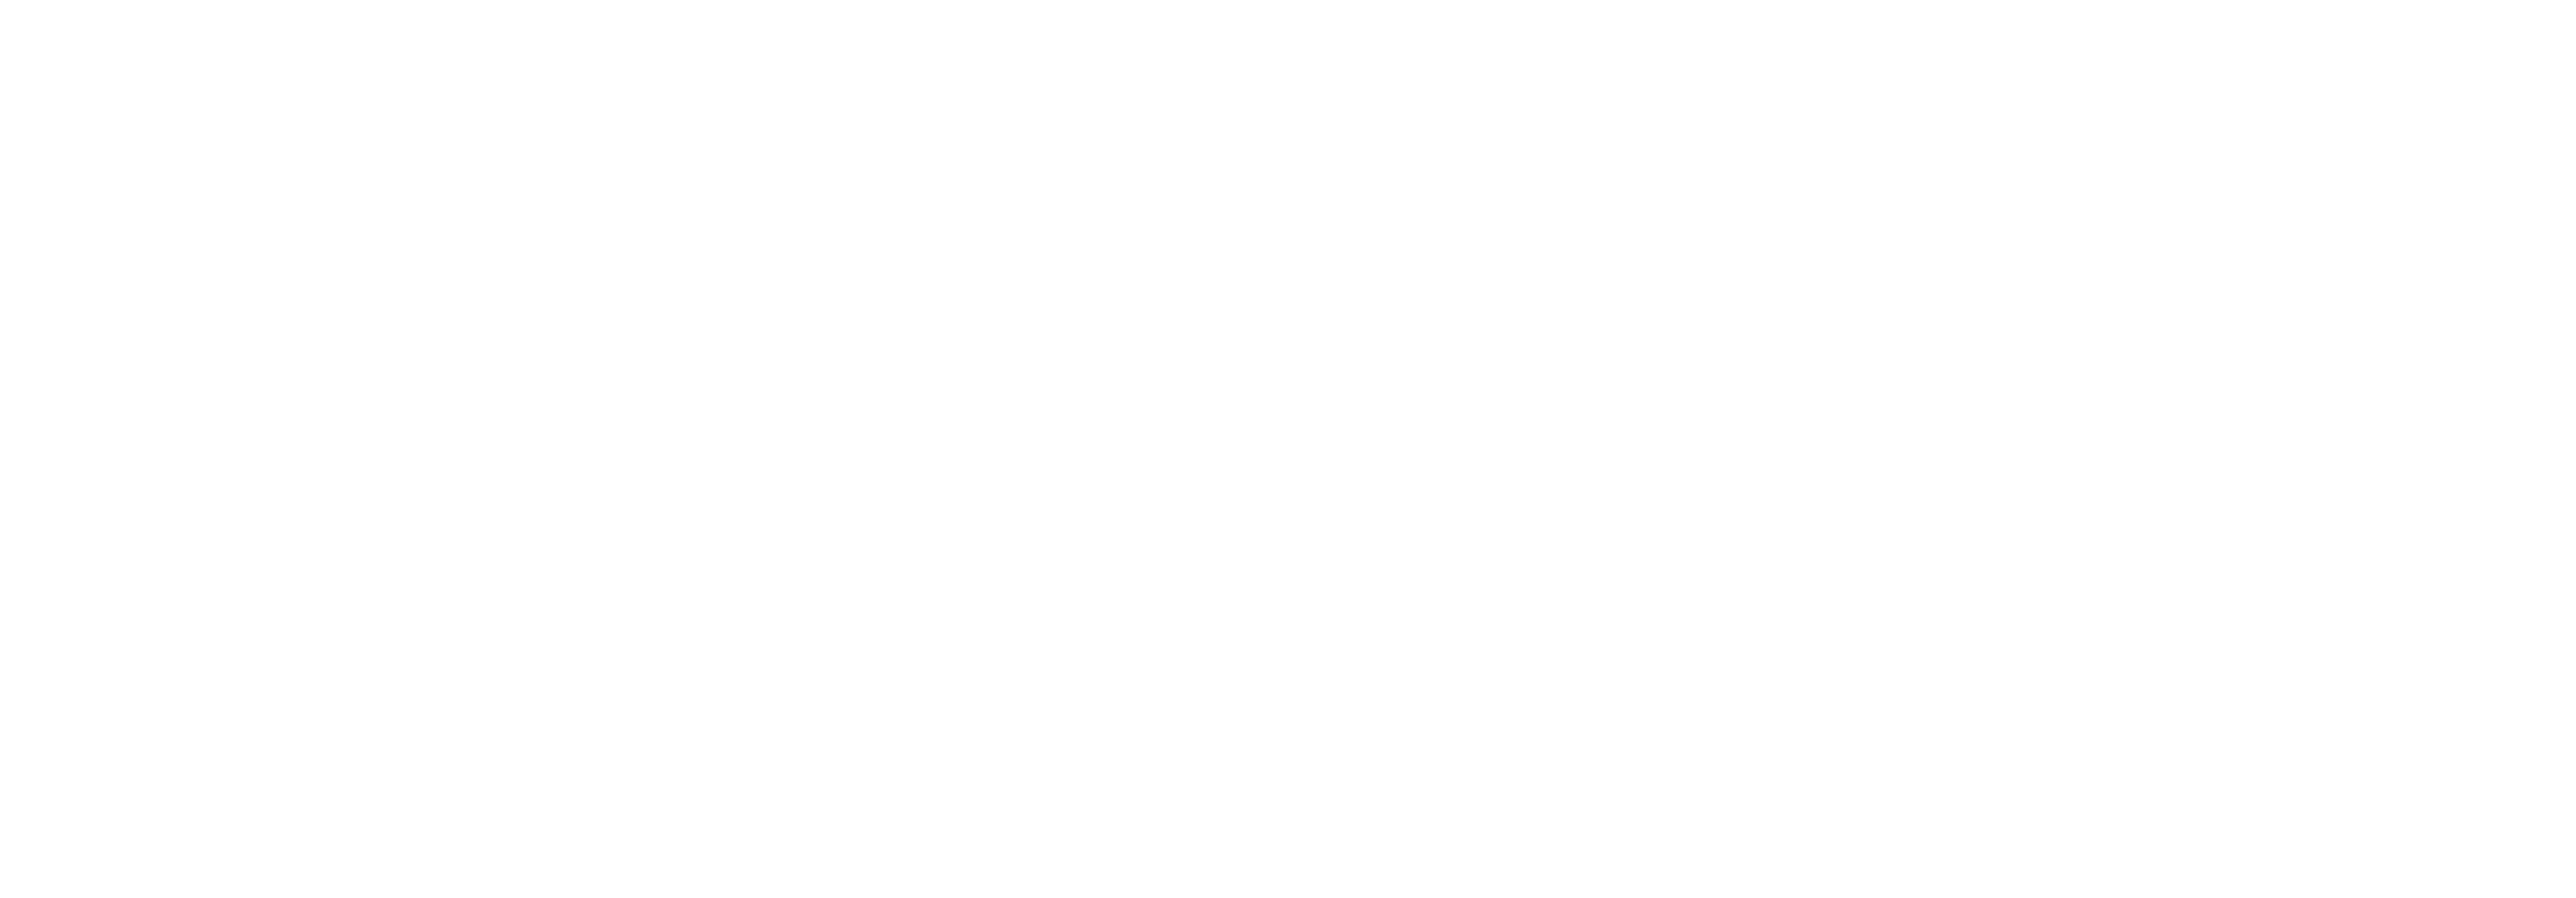
\includegraphics[
    width=19cm,
    keepaspectratio
  ]{assets/logo-transparent-bold.png}%
}\par
%\vspace{0.2cm}

% banner
{\diabatmono
\fontsize{10.8pt}{13pt}\selectfont
A Comprehensive Diabatization Toolkit for Multichromophoric Systems\par
}

% developer
\vspace{0.22cm}
{\diabatmono
\fontsize{10.2pt}{12.2pt}\selectfont
Yu-Chen Wang \textbar{} Laughtale Lab\par
}

% manual
\vspace{0.85cm}
{\rmfamily
\fontsize{36pt}{41pt}\selectfont
\bfseries
User Manual\par
}

% version
\vspace{0.3cm}
{\diabatmono
\fontsize{14pt}{15pt}\selectfont
%\bfseries
\textls[50]{PROGRAM VERSION \manualversion{}}\par
}

\end{titlepage}
\clearpage\thispagestyle{empty}\null\clearpage
\thispagestyle{empty}
\begin{center}
\vspace*{1.7cm}
\makebox[\textwidth][c]{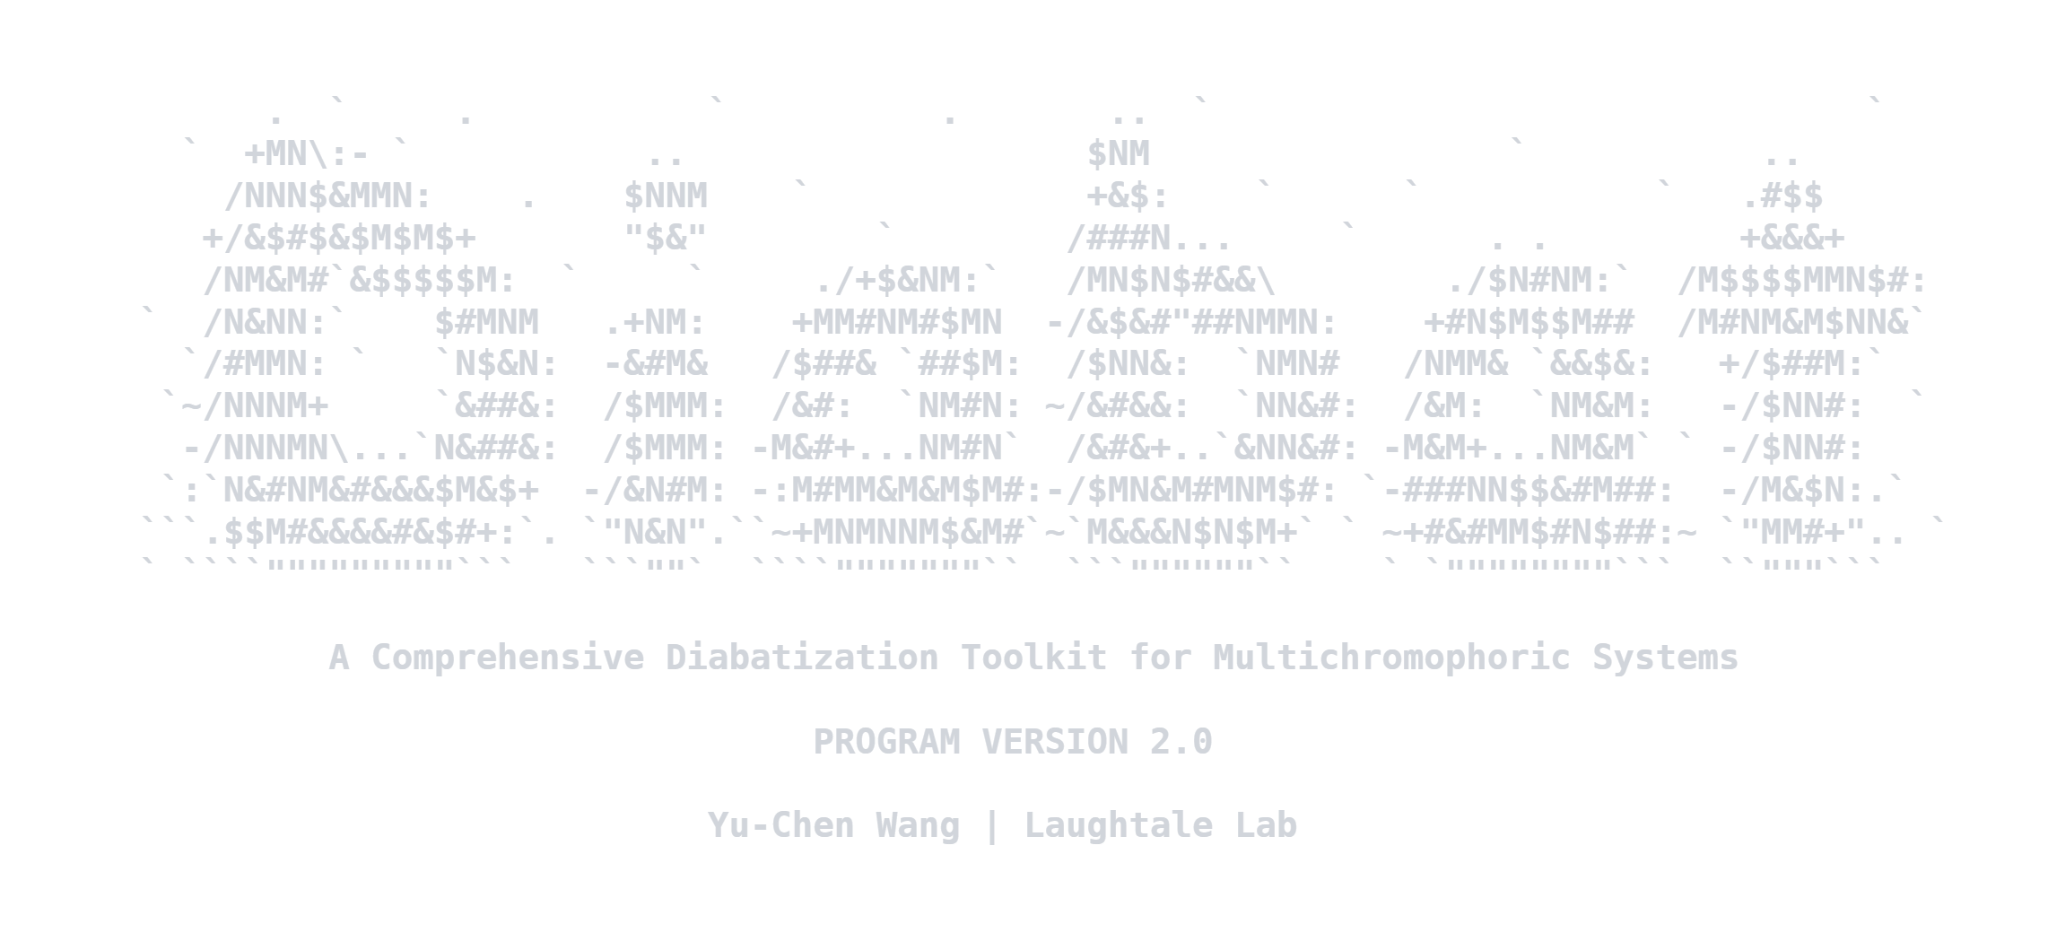
\includegraphics[width=0.94\paperwidth,keepaspectratio]{inner_cover_bold.png}}
\end{center}
\clearpage
\thispagestyle{empty}\null\clearpage

\pagestyle{plain}
\cleardoublepage
\thispagestyle{plain}
\begingroup
\small
\setstretch{1.08}
\setlength{\parindent}{0pt}
\setlength{\parskip}{0.75em}
\phantomsection\addcontentsline{toc}{chapter}{How to Cite \progname{}}
\begin{center}
{\LARGE\bfseries How to Cite Diabat}\par
\end{center}
\vspace{0.6cm}
If you use \progname{} in published work, please cite the software release article. The final journal information and DOI will be added to this manual after formal publication.

\begin{quote}
Y.-C. Wang, Y. Qin, Y. Zhao, and W. Z. Liang.\\
\textit{Diabat 2.0: A Comprehensive Diabatization Toolkit for Multichromophoric Systems.}\\
\textit{Journal of Chemical Theory and Computation}, [year], [volume], [pages].\\
DOI: [DOI to be updated].
\end{quote}

If your calculations use the fragment particle-hole densities (FPHD) method, please also cite the two FPHD method papers.

\begin{quote}
Y.-C. Wang, S. Feng, W. Z. Liang, and Y. Zhao.\\
\textit{Electronic Couplings for Photoinduced Charge Transfer and Excitation Energy Transfer Based on Fragment Particle--Hole Densities.}\\
\textit{J. Phys. Chem. Lett.} \textbf{2021}, \textit{12}, 1032--1039.\\
\href{https://doi.org/10.1021/acs.jpclett.0c03514}{doi:10.1021/acs.jpclett.0c03514}

\vspace{0.45em}
Y.-C. Wang, S. Feng, Y. Kong, X. Huang, W. Z. Liang, and Y. Zhao.\\
\textit{Electronic Couplings for Singlet Fission Processes Based on the Fragment Particle--Hole Densities.}\\
\textit{J. Chem. Theory Comput.} \textbf{2023}, \textit{19}, 3900--3914.\\
\href{https://doi.org/10.1021/acs.jctc.3c00243}{doi:10.1021/acs.jctc.3c00243}
\end{quote}

References for the other diabatization methods are given in the corresponding method sections.
\par\endgroup\clearpage

\clearpage
\thispagestyle{plain}
\phantomsection\addcontentsline{toc}{chapter}{Official Resources}
\vspace*{2.3cm}
\begin{center}
{\LARGE\bfseries Official Resources}\par\vspace{1.9cm}
{\large\bfseries Software Repository}\par\vspace{0.3cm}
\url{https://github.com/laughtale-lab/diabat}\par\vspace{1.6cm}
{\large\bfseries Online User Manual}\par\vspace{0.3cm}
\url{https://laughtale-lab.github.io/diabat-manual}\par\vspace{0.35cm}
\end{center}\clearpage

\pagestyle{plain}
\tableofcontents
\clearpage
\pagestyle{fancy}

% The book class inserts a verso page before the first chapter when necessary.
% Keep that leaf unnumbered and without the provisional Chapter 0 running head.
\pagestyle{empty}
\mainmatter
\pagestyle{fancy}
\chapter{Introduction}\label{chap-introduction}
\section{Overview}
\progname{} is a diabatization toolkit developed by Yu-Chen Wang for research in theoretical and computational chemistry.
%\keyemph{\progname{} is a diabatization toolkit developed by Yu-Chen Wang for research in theoretical and computational chemistry.}
It is designed to provide a comprehensive and unified platform for constructing quasi-diabatic electronic states and evaluating their electronic couplings from adiabatic states obtained with external quantum chemistry programs.
Different diabatization methods are implemented within a common framework, with a uniform phase convention for the resulting quasi-diabatic states and electronic couplings.

A central focus of \progname{} is \keyemph{multistate diabatization} in \keyemph{multichromophoric systems}.
%\keyemph{A central focus of \progname{} is multistate diabatization in multichromophoric systems.}
Equipped with several advanced diabatization methods, particularly the fragment particle--hole densities (FPHD) approach, \progname{} can be applied not only to conventional nonadiabatic processes such as charge transfer, excitation energy transfer, and singlet fission in molecular dimers, but also to multichromophoric systems and processes involving less conventional charge, excitation, and spin distributions.
This enables the construction of quasi-diabatic states for a broad range of electronic-state characters without restricting the diabatization to a particular type of nonadiabatic process.
In addition to diabatization, \progname{} provides orbital and electronic-state wave-function postprocessing modules for auxiliary calculations and further analysis.

The official software repository is available at \url{https://github.com/laughtale-lab/diabat}, and the online user manual is available at
\url{https://laughtale-lab.github.io/diabat-manual}.
\manualnote{This manual describes \progname{} version~\manualversion{}.}

\section{Program modules}
\progname{} has three user modules. The corresponding input jobs are listed below.
\begin{enumerate}
\item \textbf{diabat.} This module contains the following diabatization methods.
  \begin{itemize}
  \item \texttt{\$diabat-fphd}. Fragment particle--hole densities (FPHD).
  \item \texttt{\$diabat-gmh}. Multistate generalized Mulliken--Hush (GMH).
  \item \texttt{\$diabat-fcd}. Multistate fragment charge difference (FCD).
  \item \texttt{\$diabat-fed}. Fragment excitation difference (FED).
  \item \texttt{\$diabat-fedfcd}. Multistate FED--FCD.
  \end{itemize}
%FPHD is a distinctive feature of \progname{}. It permits diabatization of multichromophoric systems without prescribing the types of quasi-diabatic states in advance, provided that the states can be distinguished by their fragment particle and hole distributions.
It also includes the \texttt{\$diabat-utils-phasefix} utility for adjusting wave-function phases relative to selected reference states. See Chapter~\ref{chap-diabat}.

\item \textbf{postorb.}
This module provides postprocessing and analysis of atomic and molecular orbitals.
It supports the calculation of various one-electron integrals, the conversion among different orbital-file formats, and the generation of real-space grid data for orbitals, electron densities, and spin densities.
See Chapter~\ref{chap-postorb}.

\item \textbf{postwfn.}
This module provides postprocessing and analysis of electronic-state wave functions based on one-particle density matrices, transition density matrices, and difference density matrices.
It supports natural-orbital analyses, the calculation of various electronic and transition properties, and the generation of real-space grid data for various densities, such as electron, transition, and difference densities.
Both adiabatic and quasi-diabatic states can be analyzed.
See Chapter~\ref{chap-postwfn}.

\end{enumerate}

\section{General workflow}
A typical calculation consists of three steps.
\begin{enumerate}
\item Use a supported external quantum chemistry program to calculate the adiabatic electronic states needed for the intended task. Depending on the calculation, one or several external calculations may be required. Retain the molecular orbital files and the files that contain the electronic-state wave-function data. The latter are usually the calculation log files.
\item Prepare a \progname{} input script such as \texttt{diabat.inp}. The script specifies the computational job, the paths of the external data files, and the options required by that job.
\item Run \progname{} with the input script and inspect the reported results. A serial calculation is started with
\begin{lst-installation}
diabat diabat.inp
\end{lst-installation}
\end{enumerate}

\section{Read this first: A quick route through this manual}\label{sec-manual-route}
Begin with the installation procedure in Section~\ref{sec-install}. Confirm that the executable is correctly installed and that the \exec{} command is available from any working directory. You can then try the following route without reading the entire manual first.

\begin{enumerate}
\item \textbf{Run your first calculation.} Section~\ref{sec-quickstart} shows how to run the distributed formaldehyde-dimer example. In about one minute, you can learn how an FPHD calculation of singlet--singlet excitation energy transfer is started and where its results are written. The complete input is reproduced in \example{chap-diabat}{fphd-fmd}.

\item \textbf{Understand the input.} Once you have run the example, read Section~\ref{sec-input-syntax} for the input-script syntax and Section~\ref{sec-statepack} to learn how external orbital files and electronic-state data are specified and read by \progname{}.
Section~\ref{sec-method-support} lists the supported external quantum chemistry interfaces and electronic-structure methods.

\item \textbf{Find the relevant job.} Chapter~\ref{chap-diabat} covers diabatization methods, Chapter~\ref{chap-postorb} covers orbital processing, and Chapter~\ref{chap-postwfn} covers electronic-state wave-function analyses. Read the section for the particular method or task you intend to use.

\item \textbf{Try more examples.} Run other distributed examples before preparing a new input script from scratch.
Their inputs illustrate how job settings vary across different calculations.

\item \textbf{Explore challenging applications.} Chapter~\ref{chap-tutorials} presents four practical applications from the release article. These examples show how the same input conventions are used to investigate more complicated electronic-state mixing and nonadiabatic processes.
\end{enumerate}

Each method section begins with a short \textbf{Background}, followed by \textbf{Job Control}, method-specific \textbf{Output Data Files}, and \textbf{Examples}. Job Control includes a keyword summary for quick lookup and detailed keyword descriptions for preparing an input. The appendices provide supplementary materials for deeper understanding of the \progname{} program.

% Citation details appear before the table of contents.

\chapter{Installation and Getting Started}\label{chap-getting-started}
\section{Download and installation}\label{sec-install}
Download the binary archive for the desired release from the \href{https://github.com/laughtale-lab/diabat/releases}{official release page}. The archive filename includes its version number. For example, the version 2.0 Linux x86\_64 release is named
\begin{lst-installation}
diabat-v2.0-linux-x86_64.tar.gz
\end{lst-installation}

The commands below illustrate installation of this release. For another release, substitute its actual archive and extracted-directory names.
\begin{lst-installation}
tar -xzf diabat-v2.0-linux-x86_64.tar.gz
cd diabat-v2.0-linux-x86_64
bash install.sh
\end{lst-installation}
The installer checks selected runtime requirements, prepares the paths used by the distributed examples, and prints the executable directory to add to \texttt{PATH}. The shell startup files are not modified automatically. Use the installation location reported by the installer when setting the path. For example,
\begin{lst-installation}
export PATH="/your/installation/diabat-v2.0-linux-x86_64/bin:$PATH"
\end{lst-installation}
The archive also contains release notes, build information, examples, and the data required by those examples. Release-specific details are recorded in \texttt{README.md} and \texttt{BUILDINFO.txt}.

\subsection{Command-line information}
Several command-line queries can be used without an input script.
\begin{lst-installation}
diabat --help
\end{lst-installation}
This command prints the available command-line options.
\begin{lst-installation}
diabat --usage
\end{lst-installation}
This command prints a concise guide to serial, MPI, OpenMP, and hybrid execution. It also summarizes OpenMP thread selection and standard-output redirection.
\begin{lst-installation}
diabat --version
\end{lst-installation}
This command prints the installed program version and basic release information.
\begin{lst-installation}
diabat --module
\end{lst-installation}
This command lists the user modules and jobs available in the installed release.
\begin{lst-installation}
diabat --show diabat-fphd
\end{lst-installation}
This command prints information for a specified job. Replace \texttt{diabat-fphd} with another job name listed by \texttt{--module}.

\subsection{Runtime libraries}\label{sec-runtime}
%The distributed executable requires compatible Intel Fortran runtime libraries, Intel Math Kernel Library (MKL) for BLAS and LAPACK, Intel MPI, and Intel OpenMP, together with standard Linux libraries. These libraries must be visible to the dynamic linker when the program starts.
The distributed executable \exec{} requires the following runtime libraries, which must be visible to the dynamic linker at startup:

\begin{itemize}[noitemsep, topsep=0pt]
  \item Compatible Intel Fortran runtime libraries.
  \item Intel Math Kernel Library (MKL) for BLAS and LAPACK.
  \item Intel MPI.
  \item Intel OpenMP runtime libraries.
  \item Standard Linux system libraries.
\end{itemize}
%These libraries must be visible to the dynamic linker when \progname{} starts.
The way these libraries are provided depends on the local computer or HPC platform. Consult the system administrator or local software documentation when the Intel runtime environment is centrally managed.

On a workstation with an Intel oneAPI installation, a common approach is to initialize the Intel environment before running the program.
\begin{lst-installation}
source /path/to/intel/oneapi/setvars.sh
\end{lst-installation}
If the required libraries are installed in nonstandard locations, their directories can instead be added to the dynamic-linker search path.
\begin{lst-installation}
export LD_LIBRARY_PATH="/path/to/intel/libs:$LD_LIBRARY_PATH"
\end{lst-installation}
On many HPC systems, the same environment is provided through site-specific modules:
\begin{lst-installation}
module avail
module load intel
module load intel-mpi
module load mkl
\end{lst-installation}
The exact module names vary between installations.

The executable can be checked with \texttt{ldd} after the environment has been loaded.
\begin{lst-installation}
ldd "$(command -v diabat)"
\end{lst-installation}
A line containing \texttt{not found} indicates that the corresponding runtime library is not visible in the current environment.

The version 2.0 Linux x86\_64 binary was compiled on Red Hat Enterprise Linux Server 7.9 with Intel Fortran Compiler \texttt{ifort 19.0.1.144} and Intel MPI 2021.7. It was linked with Intel MKL and Intel OpenMP. A newer compatible Intel runtime can often be used, although compatibility ultimately depends on the binary interfaces provided by the installed libraries. The exact build record for each release is given in its \texttt{BUILDINFO.txt}.

\section{Running a job}\label{sec-running}
\progname{} uses both MPI and OpenMP parallel programming. Serial, MPI, OpenMP, and hybrid MPI/OpenMP execution are supported. MPI parallelism is the recommended choice for most calculations.

\begin{enumerate}
\item \textbf{Serial execution.} Run the program with a single process and one thread.
\begin{lst-installation}
diabat diabat.inp
\end{lst-installation}
\item \textbf{MPI execution.} Start the required number of MPI processes using the launcher available on the local system:
\begin{lst-installation}
mpirun -np 4 diabat diabat.inp
\end{lst-installation}
In this example, four MPI processes are used.
On an HPC system, use \texttt{mpiexec} or the launcher required by the job scheduler when appropriate.
\item \textbf{OpenMP execution.} Select the number of threads through \texttt{OMP\_NUM\_THREADS} or the \texttt{-nt} option.
\begin{lst-installation}
export OMP_NUM_THREADS=4
diabat diabat.inp
\end{lst-installation}
Alternatively, the command may be written as
\begin{lst-installation}
diabat diabat.inp -nt 4
\end{lst-installation}
OpenMP is used in selected orbital-integral and cube-density calculations and in portions of the optimization for certain diabatization tasks. It does not parallelize every computational step, so MPI execution is usually more effective.
\item \textbf{Hybrid MPI/OpenMP execution.} MPI processes may each use several OpenMP threads.
\begin{lst-installation}
export OMP_NUM_THREADS=2
mpirun -np 4 diabat diabat.inp
\end{lst-installation}
Hybrid execution is generally unnecessary unless the selected calculation spends substantial time in OpenMP-enabled operations or the computing environment favors this arrangement.
\end{enumerate}

If \texttt{OMP\_NUM\_THREADS} and \texttt{-nt} are both provided, the environment variable takes precedence. The default is one OpenMP thread. The installed program prints the supported execution forms with \texttt{diabat --usage}.

\subsection{Standard output and error output}\label{sec-stdout}
\progname{} writes progress information and calculation results to standard output \texttt{stdout}. Diagnostic and error messages are sent to standard error \texttt{stderr}. Both streams normally appear in the \keyemph{terminal}.

Shell redirection can save them to separate files. For example, the following command writes normal output to \texttt{diabat.log} and error messages to \texttt{diabat.err}.
\begin{lst-installation}
diabat diabat.inp > diabat.log 2> diabat.err
\end{lst-installation}
To combine both streams in one file, use
\begin{lst-installation}
diabat diabat.inp > diabat.log 2>&1
\end{lst-installation}
These redirections can also be used for parallel runs.
Individual jobs may additionally create numerical data and wave-function files in their selected output directories.

\section{Quick Start}\label{sec-quickstart}
The binary distribution includes ready-to-run input scripts and the orbital and electronic-state data needed by its examples. The following formaldehyde-dimer calculation provides a short introduction to FPHD diabatization of singlet--singlet excitation energy transfer with TDDFT adiabatic states.

After installation, enter the example directory in the installed distribution.
\begin{lst-installation}
cd /your/installation/diabat-v2.0-linux-x86_64/examples/diabat/fphd/formaldehyde_dimer/tddft
\end{lst-installation}
The input script is named \texttt{diabat.inp}. Run it from that directory with
\begin{lst-installation}
diabat diabat.inp
\end{lst-installation}
This completes a first FPHD example without preparing any new input files. The script is reproduced in \example{chap-diabat}{fphd-fmd}, where the orbital file, selected electronic states, fragment definitions, and spatial partition are visible together. The general output files are explained in Section~\ref{sec-diabat-output}. You can run the other examples directly in their own directories or copy them to a separate working directory, provided that the file paths are updated where necessary.

The data supplied with the binary distribution originated from Gaussian and Q-Chem calculations. For redistribution, the original orbital and electronic-state files were exported again using the \texttt{postorb} and \texttt{postwfn} modules, respectively. The original external quantum chemistry input scripts are also supplied in the \texttt{data/} directory. Users with access to the corresponding quantum chemistry software may repeat those calculations to regenerate the original files and use them directly for diabatization without first re-exporting them through \progname{}. See \texttt{data/README.md} for the provenance and reproduction notes.


\chapter{Input and Electronic Structure Interfaces}\label{chap-interfaces}
\section{Input script syntax}\label{sec-input-syntax}
An input script is a plain-text file that describes the jobs to be performed and the options used by those jobs. The parser is shared by all three \progname{} modules and reports detailed diagnostics when a block, keyword, or value cannot be interpreted.

\script{chap-interfaces}{script-general-structure} shows the general structure before the individual writing rules are discussed. The illustrated file names and numerical choices are examples. Replace them with the files and options required by your calculation.
\begin{lst-script}[escapechar=@]
@\scriptnum{script-general-structure}@
# Example of the general job and nested-block structure.
$diabat-fphd
  $$statepack
    mofile = "orbitals.fchk"
    statefile = "states.log"
    state_index = 1..4
  $$
  $$frag
    num_frag = 2
    frag 1 = 1..4
    frag 2 = 5..8
  $$
$
\end{lst-script}

The general writing rules are as follows.
\begin{enumerate}
\item \textbf{Comments.} The \texttt{\#} character starts a comment. Everything after it on the same line is ignored by the parser. A comment may occupy an entire line or follow an input statement.
\item \textbf{Whitespace.} Spaces, indentation, and blank lines may be used to make the script easier to read. They do not define the block hierarchy. Indentation is therefore recommended for readability but is not required by the parser.
\item \textbf{Blocks.} Computational tasks and structured groups of options are written as blocks. The number of leading dollar signs gives the block level. A first-level job begins with one dollar sign. A nested second-level block begins with two dollar signs and a third-level block begins with three. A block ends with a line containing the same number of dollar signs used to open it. A nested block must be completely contained inside its parent block.
\item \textbf{Job and block names.} The block name follows the opening dollar signs. Hyphens may be part of a job name. For example, \texttt{\$diabat-fphd} selects the FPHD diabatization job. Use \texttt{diabat --module} to list available jobs and \texttt{diabat --show job\_name} to inspect a selected job.
\item \textbf{Keywords.} A keyword is written as \texttt{name = value}. The keyword must appear in a block that accepts it. The parser reports an error when a known keyword is placed in the wrong block or when a block contains an unsupported keyword.
\item \textbf{Character strings.} Character values may be written without quotes, with single quotes, or with double quotes when the corresponding keyword accepts a string. The examples in this manual use double quotes. Quoting is particularly useful for file paths and other values that contain spaces or characters that could otherwise be ambiguous.
\item \textbf{Logical values.} Logical keywords use \texttt{.true.} or \texttt{.false.}.
\item \textbf{Integer sequences.} Keywords such as \keyref{key-statepack-state_index}{state\_index}, \texttt{ao\_id}, \texttt{mo\_id}, fragment atom lists, and state sets use the common integer-sequence parser. Individual integers may be separated by commas. A consecutive inclusive range can be written as \texttt{i..j} or \texttt{i:j}. An explicit step is written as \texttt{i:j:step}. These forms may be mixed in one value. For example,
\begin{lst-script}
state_index = 1, 3..5, 8:12:2, 20
\end{lst-script}
selects \texttt{1, 3, 4, 5, 8, 10, 12, 20}. The values in a sequence may be listed in any order. An inclusive range may run upward or downward when its step has the appropriate sign. A zero step is invalid. Individual keywords may impose additional lower or upper bounds on the integers they accept.
\item \textbf{Several jobs in one script.} A script may contain more than one first-level job block. They are parsed as independent jobs in the order defined by the program. Input files supplied to one job are not implicitly inherited by another job.
\end{enumerate}

The parser checks block structure, keyword placement, allowed values, required options, and many relations between input items. When a script is rejected, read the first diagnostic written to standard error and correct the reported problem before interpreting later messages. This behavior is also discussed in Appendix~\ref{app-troubleshooting}.

\subsection{Keyword value types}
\label{sec-keyword-value-types}

A keyword value has one of six basic data types. The type accepted by each keyword is given in its detailed description. Keyword-specific restrictions, such as allowed ranges or the required number of values, apply in addition to the general syntax described below.

\begin{enumerate}

\item \textbf{Integers.}
An integer value is written as a whole number, for example,
\begin{lst-script}
num_frag = 4
\end{lst-script}
Whether zero or negative values are allowed depends on the individual keyword.

\item \textbf{Real numbers.}
A real value may be written in decimal or scientific notation. For example,
\begin{lst-script}
svdmin = 0.0001
jacobi_thr = 1.0e-8
\end{lst-script}
The accepted numerical range is determined by the individual keyword.

\item \textbf{Logical values.}
A logical value is written as \texttt{.true.} or \texttt{.false.}. For example,
\begin{lst-script}
partial_diag = .false.
\end{lst-script}

\item \textbf{Character strings.}
A character value may be written without quotes or enclosed in single or double quotes. The examples in this manual generally use double quotes. Quoting is particularly useful for file paths and other values containing spaces or characters that could otherwise be ambiguous. For example,
\begin{lst-script}
method = "TDDFT"
outdir = "fphd.out"
\end{lst-script}

\item \textbf{Integer sequences.}
An integer sequence consists of individual integers, ranges, or a mixture of both. Individual values are separated by commas. A consecutive inclusive range may be written as \texttt{i..j} or \texttt{i:j}, and a range with an explicit step as \texttt{i:j:step}. For example,
\begin{lst-script}
state_index = 1, 3..5, 8:12:2, 20
\end{lst-script}
selects \texttt{1, 3, 4, 5, 8, 10, 12, 20}. The values may be listed in any order. A range may run upward or downward when the step has the appropriate sign. A zero step is invalid.

\item \textbf{Real sequences.}
A real sequence is written as a comma-separated list of real values. For example,
\begin{lst-script}
refnp = 0.6, 0.7
\end{lst-script}
The required number of values and their allowed ranges are specified by the individual keyword.

\end{enumerate}
\section{External electronic-structure data}

\progname{} is an independent diabatization toolkit that operates on electronic-structure data obtained from external quantum chemistry calculations. In general, two types of external data are required.

The first is a molecular orbital (MO) file, which provides the molecular geometry, atomic-orbital (AO) basis, MOs, and related orbital information required to interpret the electronic states.
The second is an electronic-state data file based on the corresponding orbital representation.
It contains the electronic-state energies together with the wave-function information required by \progname{}, such as excitation amplitudes or configuration coefficients.
This file is usually the output or log file of the external quantum chemistry calculation.

For quantum-chemistry programs that print truncated wave functions by default, the external calculation should be configured to output sufficiently complete excitation amplitudes or configuration coefficients. Omitting significant contributions may introduce non-negligible errors to the density matrices and other quantities constructed from the electronic states.

Sections~\ref{sec-mofiles} and~\ref{sec-statepack} describe how molecular orbital files and electronic-state data files are specified and read by \progname{}, respectively. Section~\ref{sec-method-support} summarizes the external quantum chemistry interfaces supported in the current version.
\section{Molecular orbital files}\label{sec-mofiles}
The \keyref{key-statepack-mofile}{mofile} keyword specifies the file from which \progname{} reads the molecular geometry, atomic orbital (AO) basis, and molecular orbitals (MOs). Use a supported formatted-checkpoint or Molden-style file produced from the external calculation. An orbital file path may be absolute or relative to the working directory.
\begin{lst-script}[escapechar=@]
@\scriptnum{script-single-mofile}@
mofile = "path/to/orbitals.fchk"
\end{lst-script}
\keyword
{key-statepack-mofile}{mofile}{Path of a supported molecular orbital data file. The orbitals, atom sequence, and AO basis must be compatible with the electronic states selected for the task.}{\OpRequired{} when an orbital file is needed}{\OpString}{None}{Readable supported orbital data file}{Use the orbital file belonging to the corresponding external quantum chemistry calculation.}{mofile = "orbitals.fchk"}

For \texttt{postorb}, the \texttt{\$\$mopack} block can contain several orbital files when required by a particular job. The \texttt{mopack} block is \emph{not} used inside \texttt{statepack}. An electronic-state package instead has its own \keyref{key-statepack-mofile}{mofile} value, as described in Section~\ref{sec-statepack}.
\begin{lst-script}[escapechar=@]
@\scriptnum{script-mopack}@
$postorb
  $$mopack
    num_file = 2
    mofile 1 = "file_1.fchk"
    mofile 2 = "file_2.fchk"
  $$
  print_mo = .true.
$
\end{lst-script}

\subsection*{Mopack keywords}
The \texttt{mopack} form is used only by \texttt{postorb}. The following entries describe its numbered orbital-file list.
\begin{keywordoverview}
\keyitem{key-mopack-num_file}{num\_file}{Number of orbital files in the package.}
\keyitem{key-mopack-mofile_i}{mofile i}{Path of each numbered orbital file.}
\end{keywordoverview}
\keyword
{key-mopack-num_file}{num\_file}{Number of numbered orbital-file entries in the \texttt{mopack} block.}{\OpRequired}{\OpInt}{None}{Positive integer}{Set this to the exact number of \texttt{mofile i} entries that follow.}{num\_file = 2}
\keyword
{key-mopack-mofile_i}{mofile i}{Path of orbital file number \texttt{i} in a \texttt{mopack}. The index runs consecutively from 1 through \texttt{num\_file}.}{\OpRequired}{\OpString}{None}{Readable supported orbital data file}{Keep the numbered entries consecutive and use paths valid from the working directory.}{mofile 1 = "file\_1.fchk"}

\section{Electronic-state file packages}\label{sec-statepack}
A \texttt{\$\$statepack} block specifies which electronic states to load and where to find their external quantum chemistry data. For one calculation, place the orbital file, electronic-state data file, and state selection inside the same block, as in \script{chap-interfaces}{script-statepack-single}.
\begin{lst-script}[escapechar=@]
@\scriptnum{script-statepack-single}@
$$statepack
  mofile = "orbitals.fchk"
  statefile = "states.log"
  state_index = 1..5
  method = "TDDFT"
$$
\end{lst-script}

\keyref{key-statepack-mofile}{mofile} identifies the orbital file described in Section~\ref{sec-mofiles}. It supplies the geometry, AO basis, and molecular orbitals used to interpret the selected electronic states.

\keyref{key-statepack-statefile}{statefile} identifies the external electronic-state data file, normally the log produced by the quantum chemistry calculation. Both \texttt{mofile} and \texttt{statefile} accept absolute paths or paths relative to the current working directory.

\keyref{key-statepack-state_index}{state\_index} selects states in the order in which the chosen method reports them in the external data file. Indices normally begin at 1. For example, the first three excited states printed by a Gaussian TDDFT calculation are selected using \texttt{state\_index = 1..3}. The special use of index 0 with certain single-excitation methods is described below and illustrated in Section~\ref{sec-internal-ids}.

\keyref{key-statepack-method}{method} selects the method whose states are read when a single log contains more than one calculation method. \progname{} automatically identifies the external program and method when possible. If the log contains several methods and \texttt{method} is omitted, the first recognized method appearing in the file is selected. For a Q-Chem log that prints TDA states before TDDFT states, for example, \texttt{method = "TDDFT"} selects the TDDFT results and the \texttt{state\_index} numbering then begins at the first TDDFT state rather than the first TDA state. An ORCA log may similarly contain CASSCF, NEVPT2, and QD-NEVPT2 data. When the intended method is not the first one present, specify it explicitly.

\keyref{key-statepack-config_cutoff}{config\_cutoff} sets the reading cutoff for configuration coefficients or amplitudes. Keep all contributions needed for the selected analysis. Discarding important coefficients can change the resulting density matrices.

For CIS, TDA, TDHF, TDDFT, and TDA-aTB data, \keyref{key-statepack-state_index}{state\_index} may also include 0. Index 0 loads the reference ground state as an independent electronic state, while positive indices select the explicitly printed excited states in their method-specific order. Including index 0 can be useful for a charged system when the reference ground state and its excited states are to be diabatized together. For all other methods, follow the regular method-specific printed-state numbering.

\subsection{Loading states from more than one calculation}
A single outer \texttt{statepack} can contain numbered third-level packages. \script{chap-interfaces}{script-statepack-multiple} illustrates the structure used to read electronic states from two separate calculations. Here the first file supplies a reference electronic state and the second supplies the adiabatic states selected for diabatization. The paths and state lists are illustrative; the corresponding calculations must provide compatible data for the intended job.
\begin{lst-script}[escapechar=@]
@\scriptnum{script-statepack-multiple}@
$$statepack
  num_state_pack = 2
  $$$statepack-1
    mofile = "orbital_file_1.molden"
    statefile = "state_file_1.log"
    state_index = 1
    method = "CASSCF"
  $$$
  $$$statepack-2
    mofile = "orbital_file_2.molden"
    statefile = "state_file_2.log"
    state_index = 1..6
    method = "CASSCF"
  $$$
$$
\end{lst-script}
This structure makes it possible to select states from distinct files. The requirements for combining their wave functions depend on the intended calculation and are discussed in Section~\ref{sec-reading} and in the respective job chapters. For a description of the internal state numbering assigned after loading, see Section~\ref{sec-internal-ids}.

\subsection{State-package keywords}
\subsubsection*{Keyword summary}
The table below provides a compact index of the state-package keywords. Each keyword links to its detailed description.
\begin{keywordoverview}
\keyitem{key-statepack-num_state_pack}{num\_state\_pack}{Number of numbered state packages when states are read from several calculations.}
\keyitem{key-statepack-mofile}{mofile}{Orbital file. Detailed description in Section~\ref{sec-mofiles}.}
\keyitem{key-statepack-statefile}{statefile}{Electronic-state data file, normally a calculation log.}
\keyitem{key-statepack-state_index}{state\_index}{States selected from the chosen method in the external file.}
\keyitem{key-statepack-method}{method}{Optional method selection when a file includes several methods.}
\keyitem{key-statepack-config_cutoff}{config\_cutoff}{Threshold for reading configuration coefficients and amplitudes.}
\end{keywordoverview}
\subsubsection*{Detailed keyword descriptions}
The tables below give the detailed rules for the state-file selection.
\keyword
{key-statepack-num_state_pack}{num\_state\_pack}{Number of numbered \texttt{statepack-i} subblocks in a multiple-package \texttt{statepack}. This keyword is used only with the multiple-package form shown in \script{chap-interfaces}{script-statepack-multiple}.}{\OpRequired{} for a multiple-package statepack}{\OpInt}{None}{Positive integer}{Use the single-package form when all selected states come from one calculation.}{num\_state\_pack = 2}
The \keyref{key-statepack-mofile}{mofile} keyword is documented in Section~\ref{sec-mofiles}.
\keyword
{key-statepack-statefile}{statefile}{Electronic-state data file containing the selected wave-function information. Accepts an absolute path or a path relative to the working directory.}{\OpRequired}{\OpString}{None}{Existing readable state-data file}{Retain sufficient printed coefficients or excitation amplitudes.}{statefile = "states.log"}
\keyword
{key-statepack-state_index}{state\_index}{Indices of the electronic states for the selected method in the order printed by that method. For CIS, TDA, TDHF, TDDFT, and TDA-aTB, 0 may be used for the underlying reference ground state. These are external indices, not internal state IDs (Section~\ref{sec-internal-ids}).}{\OpRequired}{\OpIntseq}{None}{Integer sequence using individual values, ranges such as \texttt{i..j} or \texttt{i:j}, stepped ranges \texttt{i:j:step}, or mixtures of these forms}{Select only the desired external states and verify the chosen method. See Section~\ref{sec-input-syntax} for the general integer-sequence syntax.}{state\_index = 0, 1..3}
\keyword
{key-statepack-method}{method}{Selects results from a particular electronic-structure method from an external file that may contain several kinds of state data. The external program and earliest supported method in the file are detected automatically if omitted.}{\OpOptional}{\OpString}{Automatically detected}{Supported names in Section~\ref{sec-method-support}}{Specify this keyword when the file contains multiple methods and the intended one is not the first recognized method.}{method = "QD-NEVPT2"}
\keyword
{key-statepack-config_cutoff}{config\_cutoff}{Configuration coefficients or amplitudes at or below this absolute threshold are omitted during reading.}{\OpOptional}{\OpReal}{0}{Nonnegative real}{Keep important contributions to the target states.}{config\_cutoff = 0.0}

\section{Supported electronic-structure interfaces}\label{sec-method-support}
The public release accepts orbital and electronic-state data from Gaussian, Q-Chem, ORCA, and Amesp. Supported combinations are summarized below. The method names in the table are the exact choices recognized by the \keyref{key-statepack-method}{method} keyword. \texttt{RASCI} is a general method identifier and \texttt{RASCI1} and \texttt{RASCI2} select the corresponding RASCI-family representation when applicable.
\begin{center}
\begin{tabularx}{\textwidth}{p{0.19\textwidth} X}
\hline
Program & Supported methods \\\hline
Gaussian & \texttt{CIS}, \texttt{TDA}, \texttt{TDHF}, \texttt{TDDFT} \\
Q-Chem & \texttt{CIS}, \texttt{TDA}, \texttt{TDHF}, \texttt{TDDFT}, \texttt{RASCI}, \texttt{RASCI1}, \texttt{RASCI2} \\
ORCA & \texttt{CIS}, \texttt{TDA}, \texttt{CASSCF}, \texttt{NEVPT2}, \texttt{QD-NEVPT2} \\
Amesp & \texttt{CIS}, \texttt{TDA}, \texttt{TDHF}, \texttt{TDDFT}, \texttt{TDA-aTB} \\\hline
\end{tabularx}
\end{center}
The \keyref{key-statepack-method}{method} keyword selects a wave-function data set, not merely a label for the calculation. A single Q-Chem output may contain both CIS/TDA and TDHF/TDDFT data. An ORCA output may contain CASSCF, NEVPT2, and QD-NEVPT2 information. When several methods are printed, \keyref{key-statepack-method}{method} can select the intended one. If omitted, \progname{} reads the earliest supported method present in the file. The method identifier is used with the detected external program to select the corresponding parser. An accepted identifier does not imply that the same method is available in every external program.

For all interfaces, print sufficiently complete electronic-state coefficients or excitation amplitudes. The required quantum chemistry output settings depend on the selected method and program. The data examples in the release and the original calculation inputs in the paper data provide concrete working configurations. Omitting significant coefficients may alter the computed density matrices and electronic couplings.

\section{Consistency among electronic-state files}
\label{sec-reading}

The electronic states used in a single \progname{} job may be read from one or more external quantum chemistry calculations. When all states are obtained from the same calculation, the single-package form in \script{chap-interfaces}{script-statepack-single} is sufficient. States obtained from separate calculations are supplied through the multiple-package form in \script{chap-interfaces}{script-statepack-multiple}. The separate calculations may in some cases use different electronic-structure methods or even different quantum chemistry programs.

Whether states from different calculations can be used together depends on the operation to be performed on their wave functions. \progname{} therefore checks the consistency of the loaded states according to the requirements of the requested job before the calculation begins.

For operations involving transition density matrices or linear combinations of electronic states, the participating states must be represented by mutually compatible wave functions. In particular, they must have the same wave-function type, number of electrons, AO basis, and configuration space, together with the other basic settings required by the corresponding wave-function representation. These conditions are required because interstate quantities and linear combinations are evaluated directly between the wave functions and therefore require them to share a common electronic-structure representation.

Difference-density calculations require less restrictive consistency. A reference state and a target state may be obtained with different electronic-structure methods and may contain different numbers of electrons. They must nevertheless use the same molecular geometry, atom ordering, and AO basis so that their one-particle density matrices can be represented and compared in the same AO basis. An important example is multiple-excitation FPHD for a charged system, where a separately calculated neutral state may be used as the reference state. The reference and target calculations may then differ in electron number and electronic-structure method, while the geometry, atom ordering, and AO basis must remain consistent. See Section~\ref{sec-fphd} for the reference-state requirements specific to FPHD.

Independent quantum chemistry calculations introduce an additional issue even when their computational settings are otherwise identical. MOs obtained from separate calculations may differ by arbitrary phase factors. After the relevant states have been loaded, \progname{} compares corresponding MOs from different files and determines their relative signs. The excitation amplitudes or configuration coefficients of the associated electronic states are then adjusted consistently with these orbital-phase differences. This places states read from different files under a common orbital phase convention before interstate properties or linear combinations are evaluated.
This phase adjustment does not remove the consistency requirements described above.

In summary, the admissible combination of electronic-state files is determined by the mathematical operation required by the selected job. \progname{} applies the corresponding consistency checks automatically and rejects combinations that do not provide a compatible representation for that operation.
\section{External state indices and internal state IDs}\label{sec-internal-ids}
The \keyref{key-statepack-state_index}{state\_index} values refer to states as numbered in the selected external calculation output. After the selected states are read, \progname{} assigns consecutive \emph{internal state IDs} beginning with 1. The internal IDs follow the order in which packages and their selected states are loaded. These two numbering systems are distinct, even when their values happen to coincide.

\medskip\noindent\textbf{Example 1. A selection from one file}\par\nobreak
The following selection reads five states from one external calculation:
\begin{lst-script}[escapechar=@]
@\scriptnum{script-ids-one}@
$$statepack
  mofile = "sample.fchk"
  statefile = "sample.log"
  state_index = 1..3, 5, 7
$$
\end{lst-script}
The selected external indices 1, 2, 3, 5, and 7 receive internal IDs 1, 2, 3, 4, and 5, respectively.
\begin{center}\begin{tabular}{c|ccccc}
External \keyref{key-statepack-state_index}{state\_index} & 1 & 2 & 3 & 5 & 7 \\ \hline
Internal state ID & 1 & 2 & 3 & 4 & 5
\end{tabular}\end{center}

\medskip\noindent\textbf{Example 2. Including the reference ground state}\par\nobreak
For CIS, TDA, TDHF, TDDFT, and TDA-aTB, index 0 loads the reference ground state even though the external output normally numbers its explicitly reported excited states from 1.
\begin{lst-script}[escapechar=@]
@\scriptnum{script-ids-zero}@
$$statepack
  mofile = "sample.fchk"
  statefile = "sample.log"
  method = "TDDFT"
  state_index = 0..3
$$
\end{lst-script}
Four states are loaded. The reference ground state becomes internal state 1. The first, second, and third printed TDDFT excited states become internal states 2, 3, and 4.
\begin{center}\begin{tabular}{c|cccc}
External \keyref{key-statepack-state_index}{state\_index} & 0 & 1 & 2 & 3 \\ \hline
Internal state ID & 1 & 2 & 3 & 4
\end{tabular}\end{center}

\medskip\noindent\textbf{Example 3. States from two files}\par\nobreak
Consider a separate CASSCF reference calculation followed by a target calculation, as in the example below. The first package loads reference root 1. The second package selects target roots 2, 4, and 5. These four loaded states receive internal IDs 1 through 4 in package order, irrespective of the external root numbers.
\begin{lst-script}[escapechar=@]
@\scriptnum{script-ids-two}@
$$statepack
  num_state_pack = 2
  $$$statepack-1
    mofile = "reference.molden"
    statefile = "reference.log"
    method = "CASSCF"
    state_index = 1
  $$$
  $$$statepack-2
    mofile = "target.molden"
    statefile = "target.log"
    method = "CASSCF"
    state_index = 2, 4, 5
  $$$
$$
\end{lst-script}
\begin{center}\begin{tabular}{c|cccc}
Package & 1 & 2 & 2 & 2 \\ \hline
External \keyref{key-statepack-state_index}{state\_index} & 1 & 2 & 4 & 5 \\ \hline
Internal state ID & 1 & 2 & 3 & 4
\end{tabular}\end{center}

Certain job options use internal state IDs rather than external indices. For example, \keyref{key-fphd-refid}{refid} identifies a previously loaded reference state, and the \texttt{\$\$stateset} block (Section~\ref{sec-stateset}) specifies groups of internal states permitted to mix. Always check the loaded-state order printed in standard output when selecting these values.


\chapter{Diabatization: \texttt{diabat}}\label{chap-diabat}
\section{General background}\label{sec-diabat-common}
Adiabatic-to-diabatic (ATD) diabatization constructs quasi-diabatic states from selected adiabatic states of a molecular system. If \(\lvert\Psi_n\rangle\) are the chosen adiabatic wave functions, the resulting states are
\begin{equation}
\lvert\Phi_k\rangle=\sum_n U_{nk}\lvert\Psi_n\rangle,
\end{equation}
where $\hat{U}$ is the ATD transformation. In the adiabatic representation, the Hamiltonian is diagonal when the original adiabatic energies are used. The quasi-diabatic Hamiltonian $\hat{H}^{\mathrm{d}}$ is obtained via
\begin{equation}
\hat{H}^{\rm d}=\hat{U}^{\dagger}\hat{H}^{\rm ad}\hat{U}.
\end{equation}
Its diagonal elements are quasi-diabatic state energies and its off-diagonal elements are electronic couplings.

\progname{} implements FPHD, GMH, FCD, FED, and multistate FED--FCD. Each method selects $\hat{U}$ and idenfity the state character using a different state descriptor. Their scope and restrictions are given in the following sections. For multistate calculations, different states can have similar descriptors. The program therefore normally performs a partial Hamiltonian diagonalization within groups of states having the same assigned character. The resulting transformation and Hamiltonian should be interpreted together.
See the software release paper\cite{Diabat2026} for further theoretical details.

The program uses a common phase convention for coupling signs at a fixed nuclear geometry and Cartesian orientation.
Although this convention often leads to consistent phases between nearby geometries, it does not itself guarantee phase continuity when the nuclear geometry changes.
 Appendix~\ref{app-phase} explains the convention.
 The Phasefix utility is described in Section~\ref{sec-phasefix}.
\section{Molecular fragments and spatial partitioning}\label{sec-diabat-frag}
Fragment-based methods require the user to partition the atoms of the system into molecular fragments. An atom belongs to the fragment whose index list contains that atom. The order of indices follows the orbital file and is therefore determined by the original quantum chemistry calculation. FPHD can use more than two fragments, while the GMH, FCD, FED, and multistate FED--FCD job implementations require two fragments.

\begin{lst-script}[escapechar=@]
@\scriptnum{diabat-fragment-script}@
$$<frag>
  num_frag = 2
  frag 1 = 1..6
  frag 2 = 7..12
$$
\end{lst-script}
The physical spatial region of a fragment is defined through a population-analysis partition. \progname{} supports L\"owdin and Mulliken partitions, selected with \keyref{key-common-partition}{partition}. L\"owdin and Mulliken are the two available AO-based partitions. The user may select either scheme according to the calculation. L\"owdin is the default and is generally preferable when a more balanced distribution of the AO overlap is desired. Mulliken offers an alternative population partition when it is appropriate for the system or the analysis. Additional partitioning methods may be supported in future releases.

\section{Common job settings}\label{sec-diabat-settings}
The principal diabatization jobs use the shared electronic-state package of Section~\ref{sec-statepack} and the fragment definition of Section~\ref{sec-diabat-frag}. The following options are used by several methods. The Job Control subsection for each method links back to these entries rather than repeating their definitions.

\subsection{Common keywords}
\subsubsection*{Keyword summary}
The following table provides a compact index of the options shared by the principal diabatization jobs. Each keyword links to its detailed description below.
\begin{keywordoverview}
\keyitem{key-common-diabat_wfn}{diabat\_wfn}{Save the constructed quasi-diabatic wave functions.}
\keyitem{key-common-partition}{partition}{Select L\"owdin or Mulliken population analysis.}
\keyitem{key-common-partial_diag}{partial\_diag}{Partially diagonalize the Hamiltonian within assigned state classes.}
\keyitem{key-common-adiabatic_hamiltonian}{adiabatic\_hamiltonian}{Supply the input adiabatic Hamiltonian in eV.}
\keyitem{key-common-outdir}{outdir}{Select the output directory.}
\keyitem{key-common-tmpdir}{tmpdir}{Select the temporary directory.}
\end{keywordoverview}
\subsubsection*{Detailed keyword descriptions}
The tables below give the data type, effective default behavior, accepted values, and practical use of each shared keyword.
\keyword
{key-common-diabat_wfn}{diabat\_wfn}{Write the resulting quasi-diabatic wave functions for further analysis.}{\OpOptional}{\OpLogic}{\OpTrue}{\OpTrue{} or \OpFalse}{Keep enabled when follow-up wave-function analysis is required.}{diabat\_wfn = .true.}
\keyword
{key-common-partition}{partition}{Choose the AO-based fragment population partition.}{\OpOptional}{\OpString}{\texttt{lowdin}}{\texttt{lowdin} or \texttt{mulliken}}{Choose according to the intended population analysis. L\"owdin is generally preferred.}{partition = "lowdin"}
\keyword
{key-common-partial_diag}{partial\_diag}{Perform partial Hamiltonian diagonalization among states assigned to the same class. For a calculation with exactly two target states, this step is skipped by default unless the keyword is explicitly supplied.}{\OpOptional}{\OpLogic}{Enabled for multistate jobs. Skipped automatically for two-state jobs when omitted}{\OpTrue{} or \OpFalse}{Normally omit this keyword. Set it explicitly only when the intermediate property-localized representation or an explicitly requested two-state partial diagonalization is required.}{partial\_diag = .true.}
\keyword
{key-common-adiabatic_hamiltonian}
{adiabatic\_hamiltonian}
{Specify the file containing a user-provided adiabatic Hamiltonian to be used in place of the default diagonal matrix of selected adiabatic-state energies. The file must use the numerical data format described in Appendix~\ref{app-numfile}. It must contain a real $N\times N$ matrix following the internal ordering of the $N$ adiabatic states being diabatized. \textbf{Every matrix element must be expressed in eV.} Supplying this file changes only the adiabatic Hamiltonian and does not modify the wave functions or state descriptors.}{\OpOptional}{\OpString}{Not used}{Readable numfile containing a real matrix}{Verify the file path, state order, matrix dimension, and energy units.}{adiabatic\_hamiltonian = "Hadia.dat"}
\keyword
{key-common-outdir}{outdir}{Directory for job-specific output files.}{\OpOptional}{\OpString}{Method name followed by .out}{Writable directory path}{Use a separate directory for each case.}{outdir = "fphd.out"}
\keyword
{key-common-tmpdir}{tmpdir}{Directory for temporary files.}{\OpOptional}{\OpString}{Method name followed by .tmp}{Writable directory path}{Use an appropriate high-capacity workspace.}{tmpdir = "fphd.tmp"}

\subsection{Restricting which states may mix}\label{sec-stateset}
The optional \texttt{\$\$stateset} block defines groups of states that may mix within a diabatization. Its indices are \emph{internal state IDs}, as explained in Section~\ref{sec-internal-ids}, not the external indices selected by \keyref{key-statepack-state_index}{state\_index}. Check the state-loading order reported on standard output before using the block.
\begin{lst-script}[escapechar=@]
@\scriptnum{script-stateset}@
$$stateset
  num_state_set = 2
  set 1 = 1..3
  set 2 = 4..6
$$
\end{lst-script}
The \texttt{\$\$stateset} block is normally unnecessary and should be used only when the intended calculation requires an explicit restriction on which states may mix. When it is used, verify the reported state groups after loading.

\section{Common output data files}\label{sec-diabat-output}
Successful diabatization calculations produce the common files below in the selected output directory. Check standard output for any additional files generated by the selected job.

\outputfile{adiabatic_energies.dat}{Energies of the selected adiabatic electronic states, using the reference-state energy as zero where applicable.}
\outputfile{ATD_unitary_matrix.dat}{The transformation matrix connecting the selected adiabatic electronic states to the final quasi-diabatic states. Its ordering is essential when interpreting the corresponding Hamiltonian.}
\outputfile{diabatic_hamiltonian.dat}{The resulting quasi-diabatic Hamiltonian, including state energies and electronic couplings. Its numerical format is described in Appendix~\ref{app-numfile}.}
\outputfile{diabatic_wavefunctions.dat}{Quasi-diabatic wave-function data, when exported by the selected job.}
\outputfile{diabatic_mo.molden}{Corresponding molecular orbital data when exported together with the quasi-diabatic wave functions.}
\par\vspace{0.55\baselineskip}

Calculation progress, state loading, assignments, and diagnostics are reported to standard output. Errors are reported to standard error. These streams may be saved explicitly using the redirection described in Section~\ref{sec-stdout}. Job-specific outputs are described within each method.

\section{FPHD}\label{sec-fphd}
\subsection{Background}
The fragment particle-hole densities (FPHD) method constructs quasi-diabatic states by localizing particle and hole distributions with respect to user-defined molecular fragments~\cite{Wang-JPCL-2021-1032,Wang-JCTC-2023-3900}. The descriptors are therefore tied directly to where electrons are attached and removed. This makes FPHD useful for charge-transfer states, locally excited states, correlated triplet-pair states, and more complicated states that combine charge and excitation characters. The method does not require the user to prescribe those state types before the calculation. It does require the relevant quasi-diabatic states to be distinguishable by their fragment particle and hole distributions.

\progname{} provides two FPHD formulations. The single-excitation formulation uses transition density matrices between the target states and a reference state. The particle and hole numbers obtained from these transition densities are localized over the fragments. This formulation is appropriate for wave functions with the supported single-excitation representation, including CIS, TDA, TDHF, TDDFT, and TDA-aTB data. When such a wave-function type is loaded and \keyref{key-fphd-multiexcite}{multiexcite} is omitted, \progname{} selects the single-excitation formulation automatically.

The multiple-excitation formulation uses difference density matrices relative to the reference state. Its objective retains information that is lost when a state has substantial multiple-excitation character. It is therefore the appropriate FPHD formulation for CASSCF, RASCI-family, NEVPT2, QD-NEVPT2, and other supported wave functions that are not represented as a single excitation from one reference. In this formulation, the reference state may be obtained with a different electronic-structure method and may even have a different number of electrons. The target and reference calculations must nevertheless use the same molecular geometry and compatible AO basis so that their density matrices can be compared in a common representation.

After localization, \progname{} classifies the intermediate quasi-diabatic states from their fragment particle and hole populations. The hole number minus the particle number gives the charge change on a fragment relative to the reference. The smaller of the particle and hole populations provides a useful measure of local excitation on that fragment. These quantities allow the same classification procedure to describe conventional LE and CT states together with multiexcitonic and mixed characters. The optional \keyref{key-fphd-refnp}{refnp} and \keyref{key-fphd-refnh}{refnh} values define background particle and hole populations for this classification step. They do not alter the localization objective.

When several intermediate states have the same classified character, their particle-hole descriptors do not uniquely distinguish them. The Hamiltonian is then partially diagonalized within each class by default in a multistate calculation. This removes arbitrary mixing inside the class while retaining the distinction between different physical classes. The release article gives the formal objectives and the general classification procedure in detail~\cite{Diabat2026}. For routine use, the reference-state choice, fragment definitions, spatial partition, and selected adiabatic-state space are usually more important than the formal equations.

\subsection{Job Control}\label{sec-fphd-job}
Start an FPHD calculation using the following block. Place the \texttt{statepack} and \texttt{frag} definitions and any selected keywords inside it. These nested blocks are described in Sections~\ref{sec-statepack} and~\ref{sec-diabat-frag}.
\begin{lst-script}[escapechar=@]
@\scriptnum{script-fphd-job}@
$diabat-fphd
  # Place statepack, frag, and relevant computational options here.
$
\end{lst-script}

\subsubsection*{Keyword summary}
The table below gives a compact index of the FPHD options. Each keyword links to its detailed description. Shared diabatization keywords are included where they are commonly used with FPHD.
\begin{keywordoverview}
\keyitem{key-fphd-multiexcite}{multiexcite}{Choose the FPHD formulation or allow automatic selection.}
\keyitem{key-fphd-refid}{refid}{Reference state selected by internal ID.}
\keyitem{key-fphd-extref}{extref}{Optional external reference states for single-excitation FPHD.}
\keyitem{key-fphd-refnp}{refnp}{Baseline fragment particle numbers used in classification.}
\keyitem{key-fphd-refnh}{refnh}{Baseline fragment hole numbers used in classification.}
\keyitem{key-fphd-printspin}{print\_spin\_fphn}{Print spin-resolved fragment populations where supported.}
\keyitem{key-fphd-svdmin}{svdmin}{Transition-density singular-value threshold.}
\keyitem{key-fphd-jacobi}{jacobi\_thr}{Jacobi optimization convergence threshold.}
\keyitem{key-fphd-maxcycle}{maxcycle}{Maximum Jacobi optimization cycles.}
\keyitem{key-fphd-cyclestep}{cyclestep}{Optimization steps per Jacobi cycle.}
\keyitem{key-fphd-densitycube}{density\_cube}{Produce density cube files.}
\keyitem{key-fphd-ngrid}{ngrid}{Spatial grid size for cube output.}
\keyitem{key-common-partition}{partition}{Select L\"owdin or Mulliken population analysis.}
\keyitem{key-common-partial_diag}{partial\_diag}{Partially diagonalize states with matching characters.}
\keyitem{key-common-adiabatic_hamiltonian}{adiabatic\_hamiltonian}{Optional input Hamiltonian in eV.}
\keyitem{key-common-diabat_wfn}{diabat\_wfn}{Write the constructed quasi-diabatic wave functions.}
\keyitem{key-common-outdir}{outdir}{Output directory.}
\keyitem{key-common-tmpdir}{tmpdir}{Temporary directory.}
\end{keywordoverview}
\subsubsection*{Detailed keyword descriptions}
The tables below give the detailed descriptions and defaults of the FPHD-specific options. The shared keywords are explained in Section~\ref{sec-diabat-settings}.
\keyword
{key-fphd-multiexcite}{multiexcite}{Select the multiple-excitation rather than the single-excitation FPHD formulation. When omitted, the program determines the formulation from the loaded wave-function type.}{\OpOptional}{\OpLogic}{Automatically selected}{Logical}{Usually omit this keyword. Specify it only to override automatic selection.}{multiexcite = .true.}
\keyword
{key-fphd-refid}{refid}{Internal ID of a loaded reference state (Section~\ref{sec-internal-ids}). The reference is normally outside the states being diabatized.}{\OpOptional}{\OpInt}{Automatically use the underlying reference for single-excitation wave functions. Otherwise required}{1 to number of loaded states}{For multiple-excitation FPHD, the reference may have a different electron number, but it must share the same nuclear geometry and AO basis. Explicitly load and select a reference for CASSCF, RASCI, or related wave functions.}{refid = 1}
\keyword
{key-fphd-extref}{extref}{Additional external reference-state IDs in the single-excitation FPHD formulation.}{\OpOptional}{\OpIntseq}{None}{Internal state ID sequence}{Do not use with the multiple-excitation formulation.}{extref = 3, 5}
\keyword
{key-fphd-refnp}{refnp}{Reference baseline particle populations on the fragments used in FPHD state classification.}{\OpOptional}{\OpRealseq}{Zero for each fragment}{Exactly one real value per fragment}{Use only when background populations alter the intended classification.}{refnp = 0.6, 0.6}
\keyword
{key-fphd-refnh}{refnh}{Reference baseline hole populations on the fragments used in FPHD state classification.}{\OpOptional}{\OpRealseq}{Zero for each fragment}{Exactly one real value per fragment}{Choose together with refnp when needed.}{refnh = 0.6, 0.6}
\keyword
{key-fphd-printspin}{print\_spin\_fphn}{Print spin-resolved particle and hole populations in applicable multiple-excitation FPHD analyses.}{\OpOptional}{\OpLogic}{\OpFalse}{Logical}{Useful for open-shell systems and mixed radical--triplet states.}{print\_spin\_fphn = .true.}
\keyword
{key-fphd-svdmin}{svdmin}{Singular-value threshold used in the single-excitation transition-density formulation.}{\OpOptional}{\OpReal}{0.0001}{Real threshold}{Check sensitivity if important transition-density contributions are small.}{svdmin = 0.0001}
\keyword
{key-fphd-jacobi}{jacobi\_thr}{Jacobi-sweep convergence threshold.}{\OpOptional}{\OpReal}{$\max(10^{-8},\mathrm{fperr})$}{Nonnegative real}{Use the default unless convergence requires closer examination.}{jacobi\_thr = 1e-8}
\keyword
{key-fphd-maxcycle}{maxcycle}{Maximum number of Jacobi cycles. Setting it to zero skips the optimization.}{\OpOptional}{\OpInt}{1000}{Nonnegative integer}{Retain the default for normal FPHD runs.}{maxcycle = 1000}
\keyword
{key-fphd-cyclestep}{cyclestep}{Number of optimization steps in a Jacobi cycle. An omitted value is determined from the number of states being mixed.}{\OpOptional}{\OpInt}{$N(N+1)/2$ (computed when omitted)}{Nonnegative integer}{Normally omit this keyword. Use a custom value only when investigating convergence.}{cyclestep = 100}
\keyword
{key-fphd-densitycube}{density\_cube}{Write particle/hole or attachment/detachment spatial grid data for the constructed quasi-diabatic states.}{\OpOptional}{\OpLogic}{\OpFalse}{Logical}{Enable if the localized densities need visual inspection.}{density\_cube = .true.}
\keyword
{key-fphd-ngrid}{ngrid}{Requested spatial grid count when density cube output is enabled.}{\OpOptional}{\OpInt}{1728000}{Positive integer}{A larger grid increases computational effort and output size.}{ngrid = 1728000}

\subsection{Output Data Files}
FPHD produces the common diabatization files of Section~\ref{sec-diabat-output}. Standard output also reports the localization process, fragment particle and hole information, state classification, and subsequent partial diagonalization. The optional \keyref{key-fphd-densitycube}{density\_cube} output contains spatial particle/hole densities in the single-excitation formulation or attachment/detachment densities in the multiple-excitation formulation. When enabled and supported by the selected states, \texttt{print\_spin\_fphn} prints spin-resolved fragment populations.

\subsection{Examples}
The following five examples use the public distribution input files and its installed data. They cover single-excitation and multiple-excitation FPHD in dimers, a multimer, and a charged system. The paths and computational parameters shown in the inputs correspond to their respective distributed cases. Replace installation-specific paths if the examples were copied to another directory.

\exampleheading{1. Dimer with single excitations: formaldehyde, singlet--singlet EET (TDDFT)}
\examplepath{examples/diabat/fphd/formaldehyde_dimer/tddft/diabat.inp}
\lstinputlisting[style=diabatfile,escapechar=@]{examples/display/release/fphd-formaldehyde-tddft.lst}

\exampleheading{2. Multimer with single excitations: ethylene tetramer (TDDFT)}
\examplepath{examples/diabat/fphd/ethylene_tetramer/diabat.inp}
\lstinputlisting[style=diabatfile,escapechar=@]{examples/display/release/fphd-ethylene-tetramer.lst}

\exampleheading{3. Neutral dimer with multiple excitations: singlet water dimer (RASCI)}
\examplepath{examples/diabat/fphd/water_dimer/neutral_singlet_rasci/diabat.inp}
\lstinputlisting[style=diabatfile,escapechar=@]{examples/display/release/fphd-water-dimer-singlet-rasci.lst}

\exampleheading{4. Neutral dimer with multiple excitations: triplet water dimer (RASCI)}
\examplepath{examples/diabat/fphd/water_dimer/neutral_triplet_rasci/diabat.inp}
\lstinputlisting[style=diabatfile,escapechar=@]{examples/display/release/fphd-water-dimer-triplet-rasci.lst}

\exampleheading{5. Charged dimer with multiple excitations: asymmetric cationic ethylene dimer (RASCI)}
\examplepath{examples/diabat/fphd/ethylene_dimer/asymmetric_cationic/rasci/diabat.inp}
\lstinputlisting[style=diabatfile,escapechar=@]{examples/display/release/fphd-cationic-ethylene-rasci.lst}

\section{GMH}\label{sec-gmh}
\subsection{Background}
The generalized Mulliken--Hush (GMH) method constructs quasi-diabatic states for charge-transfer problems based on molecular dipole moments~\cite{Cave-CPL-1996-p15,Yang-JCP-2013-p154104}. Its physical premise is that a charge-localized representation can be characterized by large differences in permanent dipole moment and vanishingly small transition dipole moments between different quasi-diabatic states. The original formulation was introduced for a two-state donor--acceptor problem. The implementation in \progname{} follows the multistate extension and can treat more than two adiabatic states within a two-fragment model.

For the user-defined fragments, \progname{} defines the charge-transfer direction from the center of mass of fragment 2 toward the center of mass of fragment 1. Permanent and transition dipole moments in the adiabatic basis are projected on this direction. Diagonalization of the projected dipole matrix produces an intermediate representation in which the projected transition dipole moments between different states vanish. The resulting projected permanent dipoles provide the descriptor used for state classification.

For a neutral system, the projected permanent dipole of each intermediate state is divided by the center-of-mass distance and the elementary positive charge, which yields an effective charge-transfer number and is used for identifying states. Values of at least 0.5 and at most -0.5 identify the two opposite CT directions. Values between these limits are treated as non-CT states. For a charged system, the total molecular charge also contributes to the permanent dipole. \progname{} removes this contribution by placing a fictitious charge equal to the total system charge at the center of mass of fragment 1 before the effective CT number is evaluated.
%This treatment avoids relying on a separately supplied ground-state dipole and is suitable for the charged two-fragment cases supported by the implementation.

When more than two states are involded in diabatization, several states may belong to the same CT class and the dipole descriptor itself cannot distinguish them uniquely. The Hamiltonian is then partially diagonalized within each assigned class. The \keyref{key-common-partial_diag}{partial\_diag} keyword controls this step. GMH is intended for charge-transfer problems. It should not be used as an excitation-energy-transfer diabatization method merely because a numerical transformation can be obtained.

\subsection{Job Control}
Start the job with the following first-level block. Add the \texttt{statepack} and \texttt{frag} blocks described in Sections~\ref{sec-statepack} and~\ref{sec-diabat-frag}.
\begin{lst-script}[escapechar=@]
@\scriptnum{script-gmh-job}@
$diabat-gmh
  # Place statepack, frag, and relevant computational options here.
$
\end{lst-script}
\subsubsection*{Keyword summary}
The following table lists the keywords commonly used in a GMH job. The links lead to the detailed definitions given earlier in the manual.
\begin{keywordoverview}
\keyitem{key-statepack-statefile}{statefile}{Electronic-state data file in \texttt{statepack}.}
\keyitem{key-common-adiabatic_hamiltonian}{adiabatic\_hamiltonian}{Read an optional adiabatic Hamiltonian in eV.}
\keyitem{key-common-partial_diag}{partial\_diag}{Control partial diagonalization within state classes.}
\keyitem{key-common-diabat_wfn}{diabat\_wfn}{Write the constructed quasi-diabatic wave functions.}
\keyitem{key-common-outdir}{outdir}{Set the output directory.}
\keyitem{key-common-tmpdir}{tmpdir}{Set the temporary directory.}
\end{keywordoverview}
\subsubsection*{Detailed keyword descriptions}
GMH has no additional method-specific keywords. The electronic-state package is described in Section~\ref{sec-statepack}. Fragment definition is described in Section~\ref{sec-diabat-frag}. Shared diabatization options are described in Section~\ref{sec-diabat-settings}.
\subsection{Output Data Files}
Besides the common output files in Section~\ref{sec-diabat-output}, the job also writes the projected dipole matrix in the original adiabatic representation.
\outputfile{property_matrix/dipole_mat.dat}{The matrix of permanent and transition dipole moments projected onto the charge-transfer direction in the original adiabatic representation. The diagonal elements are projected permanent dipoles, and the off-diagonal elements are projected transition dipoles.}
\par\vspace{0.55\baselineskip}
The standard output also reports the derived CT descriptors and, for multistate calculations, the resulting state classes.

\subsection{Examples}
The following input scripts are taken from the public distribution. Check the existence of the corresponding data files before running the scripts.

\exampleheading{Donor--acceptor dimer, TDDFT}
\examplepath{examples/diabat/gmh/donor_acceptor/diabat.inp}
\lstinputlisting[style=diabatfile,escapechar=@]{examples/display/release/gmh-donor_acceptor.lst}

\exampleheading{Cationic asymmetric ethylene dimer, CIS}
\examplepath{examples/diabat/gmh/asymmetric_ethylene_dimer/cis/diabat.inp}
\lstinputlisting[style=diabatfile,escapechar=@]{examples/display/release/gmh-asymmetric_ethylene_dimer-cis.lst}

\section{FCD}\label{sec-fcd}
\subsection{Background}
The fragment charge difference (FCD) method constructs charge-localized quasi-diabatic states from the difference in electronic charge assigned to two molecular fragments~\cite{Voityuk-JCP-2002-p5607,Yang-JCP-2013-p154104}. In contrast to GMH, FCD does not require a dipole-projection direction. The descriptor is built directly from fragment-resolved one-particle density and transition-density information together with the nuclear charges of the two fragments.

For each pair of adiabatic states, \progname{} evaluates a charge-difference matrix. Its diagonal elements are the charge difference between the two fragments for the individual adiabatic states. Its off-diagonal elements contain the corresponding transition-density contribution. Diagonalizing this matrix gives an intermediate representation that maximizes separation with respect to the fragment charge difference. The eigenvalues of the descriptor matrix are then used to identify the physical direction of charge localization.

The implementation follows a multistate treatment. To use the same classification procedure for neutral and charged systems, \progname{} shifts the descriptor eigenvalues by the total molecular charge in units of the elementary charge. A shifted value below -1 identifies electron transfer from fragment 2 to fragment 1. A shifted value above 1 identifies the opposite transfer direction. Intermediate values are treated as non-CT character. When several states belong to the same class, the Hamiltonian is partially diagonalized within that class to remove mixing that the charge-difference descriptor alone does not determine.

The public implementation accepts multiple adiabatic states but uses exactly two molecular fragments. FCD is intended for charge-transfer problems. For excitation energy transfer without the corresponding charge-separation character, FED or another suitable method should be used instead.

\subsection{Job Control}
Start the job with the following first-level block. Add the \texttt{statepack} and \texttt{frag} blocks described in Sections~\ref{sec-statepack} and~\ref{sec-diabat-frag}.
\begin{lst-script}[escapechar=@]
@\scriptnum{script-fcd-job}@
$diabat-fcd
  # Place statepack, frag, and relevant computational options here.
$
\end{lst-script}
\subsubsection*{Keyword summary}
The following table lists the keywords commonly used in an FCD job.
\begin{keywordoverview}
\keyitem{key-statepack-statefile}{statefile}{Electronic-state data file in \texttt{statepack}.}
\keyitem{key-common-partition}{partition}{Select L\"owdin or Mulliken fragment populations.}
\keyitem{key-common-adiabatic_hamiltonian}{adiabatic\_hamiltonian}{Read an optional adiabatic Hamiltonian in eV.}
\keyitem{key-common-partial_diag}{partial\_diag}{Control partial diagonalization within state classes.}
\keyitem{key-common-diabat_wfn}{diabat\_wfn}{Write the quasi-diabatic wave functions.}
\keyitem{key-common-outdir}{outdir}{Set the output directory.}
\keyitem{key-common-tmpdir}{tmpdir}{Set the temporary directory.}
\end{keywordoverview}
\subsubsection*{Detailed keyword descriptions}
FCD has no additional method-specific keywords. The shared input and output controls are described in Sections~\ref{sec-statepack}, \ref{sec-diabat-frag}, and~\ref{sec-diabat-settings}.
\subsection{Output Data Files}
Besides the common output files in Section~\ref{sec-diabat-output}, the job writes the fragment charge matrices in the adiabatic representation to the \texttt{property\_matrix/} subdirectory.
\outputfile{property_matrix/Q1.dat}{Fragment-1 charge matrix.}
\outputfile{property_matrix/Q2.dat}{Fragment-2 charge matrix.}
\outputfile{property_matrix/dQ.dat}{Fragment charge-difference matrix used by FCD.}
\par\vspace{0.55\baselineskip}
The standard output also reports the CT descriptors and the resulting state classes.

\subsection{Examples}
The following input scripts are taken from the public distribution. Install the corresponding data before running them.

\exampleheading{Donor--acceptor dimer, TDDFT}
\examplepath{examples/diabat/fcd/donor_acceptor/diabat.inp}
\lstinputlisting[style=diabatfile,escapechar=@]{examples/display/release/fcd-donor_acceptor.lst}

\exampleheading{Cationic asymmetric ethylene dimer, CIS}
\examplepath{examples/diabat/fcd/asymmetric_ethylene_dimer/cis/diabat.inp}
\lstinputlisting[style=diabatfile,escapechar=@]{examples/display/release/fcd-asymmetric_ethylene_dimer-cis.lst}

\section{FED}\label{sec-fed}
\subsection{Background}
The fragment excitation difference (FED) method was developed for excitation energy transfer between two molecular fragments~\cite{Hsu-JPCC-2008-p1204}. Its descriptor measures how strongly the electronic excitation is localized on one fragment rather than the other. The excitation population is obtained from the change in the one-particle density relative to a reference state. A physically useful FED representation maximizes the difference between the excitation populations of the two fragments.

The standalone FED job in \progname{} implements the conventional two-state formulation. Exactly two target adiabatic states are included in one FED transformation. For a general electronic-state representation, the program varies the two-state mixing angle and searches for the transformation that maximizes the absolute difference between the two FED descriptors. For single-excitation theories, the transition density between two excited states can be separated into attachment-like and detachment-like contributions. This gives an interstate excitation-difference quantity and permits an equivalent matrix treatment.

A reference state is required because the excitation descriptor is defined from a density change. For CIS, TDA, TDHF, TDDFT, and TDA-aTB wave functions, the underlying reference ground state can be used automatically when no loaded reference is selected. For other wave-function types, the reference must be loaded explicitly and selected with \keyref{key-fphd-refid}{refid}. The reference and target calculations must use the same molecular geometry and AO basis. Other computational details may differ when the resulting density matrices remain compatible.

FED should be used for two-fragment excitation-energy-transfer problems. It is distinct from FCD, which uses charge difference and targets charge transfer. A multistate excitation-difference calculation is available through the \texttt{diabat-fedfcd} job with the FCD contribution disabled.

\subsection{Job Control}
Start the job with the following first-level block. Add the \texttt{statepack} and \texttt{frag} blocks described in Sections~\ref{sec-statepack} and~\ref{sec-diabat-frag}.
\begin{lst-script}[escapechar=@]
@\scriptnum{script-fed-job}@
$diabat-fed
  # Place statepack, frag, and relevant computational options here.
$
\end{lst-script}
\subsubsection*{Keyword summary}
The following table lists the principal keywords used in an FED job.
\begin{keywordoverview}
\keyitem{key-fphd-refid}{refid}{Select an explicitly loaded reference by internal state ID.}
\keyitem{key-common-partition}{partition}{Select L\"owdin or Mulliken fragment populations.}
\keyitem{key-common-partial_diag}{partial\_diag}{Control the final partial diagonalization.}
\keyitem{key-common-adiabatic_hamiltonian}{adiabatic\_hamiltonian}{Read an optional adiabatic Hamiltonian in eV.}
\keyitem{key-common-diabat_wfn}{diabat\_wfn}{Write the quasi-diabatic wave functions.}
\keyitem{key-common-outdir}{outdir}{Set the output directory.}
\keyitem{key-common-tmpdir}{tmpdir}{Set the temporary directory.}
\end{keywordoverview}
\subsubsection*{Detailed keyword descriptions}
The \keyref{key-fphd-refid}{refid} keyword uses an internal state ID as explained in Section~\ref{sec-internal-ids}. The general meaning of the keyword is given in the FPHD table in Section~\ref{sec-fphd-job}. The reference may be calculated with a different electronic-structure method or electron number, provided that its molecular geometry and AO basis are compatible with those of the target states. The standalone FED job uses exactly two target adiabatic states. Shared options are described in Section~\ref{sec-diabat-settings}.
\subsection{Output Data Files}
Besides the common output files in Section~\ref{sec-diabat-output}, the job writes the fragment excitation matrices in the adiabatic representation to the \texttt{property\_matrix/} subdirectory.
\outputfile{property_matrix/E1.dat}{Fragment-1 excitation matrix.}
\outputfile{property_matrix/E2.dat}{Fragment-2 excitation matrix.}
\outputfile{property_matrix/dE.dat}{Fragment excitation-difference matrix used by FED.}
\par\vspace{0.55\baselineskip}
The standard output also reports the selected FED transformation and the excitation differences.

\subsection{Examples}
The following input scripts are taken from the public distribution. Install the corresponding data before running them.

\exampleheading{Formaldehyde dimer, TDDFT}
\examplepath{examples/diabat/fed/formaldehyde_dimer/tddft/diabat.inp}
\lstinputlisting[style=diabatfile,escapechar=@]{examples/display/release/fed-formaldehyde_dimer-tddft.lst}

\exampleheading{Water dimer, RASCI}
\examplepath{examples/diabat/fed/water_dimer/neutral_singlet_rasci/diabat.inp}
\lstinputlisting[style=diabatfile,escapechar=@]{examples/display/release/fed-water_dimer-neutral_singlet_rasci.lst}

\section{Multistate FED--FCD}\label{sec-fedfcd}
\subsection{Background}
Multistate FED--FCD combines the fragment excitation difference and fragment charge difference descriptors for two-fragment systems in which excitation energy transfer and photoinduced charge transfer can coexist and mix~\cite{Nottoli-PR-2018-p215}. The two descriptors separate different physical characters in complementary ways. A charge-transfer state has a large fragment charge difference and normally a much smaller excitation difference. A locally excited state has a large excitation difference and a much smaller charge difference.

The calculation begins with the charge-difference and excitation-difference matrices for the selected adiabatic states. It then forms a combined descriptor from the square of the excitation-difference matrix and the square of the charge-difference matrix. Diagonalization of this descriptor separates an initial CT block from an initial LE block. Within the CT block, the charge-difference descriptor separates the two directions of charge transfer. Within the LE block, the excitation-difference descriptor separates excitation localized on fragment 1 from excitation localized on fragment 2.

This procedure gives four physical classes in the full calculation. States within a class may still have similar descriptor values, so the Hamiltonian is partially diagonalized within each class to remove the remaining arbitrary mixing. The resulting transformation can therefore describe coherent mixing among LE and CT characters while retaining a clear distinction between the classes defined by the two descriptors.

The complete excitation-difference matrix requires interstate quantities that are available for the supported single-excitation wave-function representations. The multistate FED--FCD implementation is therefore restricted to single-excitation theories. The user may omit the FED contribution with \keyref{key-fedfcd-skip_fed}{skip\_fed} and obtain the corresponding multistate FCD treatment. The FCD contribution may instead be omitted with \keyref{key-fedfcd-skip_fcd}{skip\_fcd} to obtain a multistate FED treatment. Both contributions cannot be disabled in the same job.

\subsection{Job Control}
Start the job with the following first-level block. Add the \texttt{statepack} and \texttt{frag} blocks described in Sections~\ref{sec-statepack} and~\ref{sec-diabat-frag}.
\begin{lst-script}[escapechar=@]
@\scriptnum{script-fedfcd-job}@
$diabat-fedfcd
  # Place statepack, frag, and relevant computational options here.
$
\end{lst-script}
\subsubsection*{Keyword summary}
The following table lists the method-specific controls and the most frequently used shared options.
\begin{keywordoverview}
\keyitem{key-fedfcd-skip_fed}{skip\_fed}{Omit the FED descriptor and perform multistate FCD.}
\keyitem{key-fedfcd-skip_fcd}{skip\_fcd}{Omit the FCD descriptor and perform multistate FED.}
\keyitem{key-common-partition}{partition}{Select L\"owdin or Mulliken fragment populations.}
\keyitem{key-common-partial_diag}{partial\_diag}{Control partial diagonalization within state classes.}
\keyitem{key-common-adiabatic_hamiltonian}{adiabatic\_hamiltonian}{Read an optional adiabatic Hamiltonian in eV.}
\keyitem{key-common-diabat_wfn}{diabat\_wfn}{Write the quasi-diabatic wave functions.}
\keyitem{key-common-outdir}{outdir}{Set the output directory.}
\keyitem{key-common-tmpdir}{tmpdir}{Set the temporary directory.}
\end{keywordoverview}
\subsubsection*{Detailed keyword descriptions}
The shared keywords are explained in Section~\ref{sec-diabat-settings}. The two method-specific switches are given below.
\keyword
{key-fedfcd-skip_fed}{skip\_fed}{Omit the FED descriptor and carry out the corresponding multistate FCD calculation.}{\OpOptional}{\OpLogic}{\OpFalse}{\OpTrue{} or \OpFalse}{Keep this false for the combined FED--FCD calculation. Do not set both skip flags to true.}{skip\_fed = .false.}
\keyword
{key-fedfcd-skip_fcd}{skip\_fcd}{Omit the FCD descriptor and carry out the corresponding multistate FED calculation.}{\OpOptional}{\OpLogic}{\OpFalse}{\OpTrue{} or \OpFalse}{Keep this false for the combined FED--FCD calculation. Do not set both skip flags to true.}{skip\_fcd = .false.}
\subsection{Output Data Files}
Besides the common output files in Section~\ref{sec-diabat-output}, the job writes the descriptor matrices in the adiabatic representation to the \texttt{property\_matrix/} subdirectory.
\outputfile{property_matrix/Q1.dat}{Fragment-1 charge matrix.}
\outputfile{property_matrix/Q2.dat}{Fragment-2 charge matrix.}
\outputfile{property_matrix/dQ.dat}{Fragment charge-difference matrix.}
\outputfile{property_matrix/E1.dat}{Fragment-1 excitation matrix.}
\outputfile{property_matrix/E2.dat}{Fragment-2 excitation matrix.}
\outputfile{property_matrix/dE.dat}{Fragment excitation-difference matrix.}
\outputfile{property_matrix/D.dat}{Combined descriptor matrix used to separate CT and LE blocks.}
\par\vspace{0.55\baselineskip}
The standard output reports whether the combined or reduced calculation was selected and gives the resulting state classes.

\subsection{Examples}
The following input scripts are taken from the public distribution. Install the corresponding data before running them.

\exampleheading{Donor--acceptor dimer, TDDFT}
\examplepath{examples/diabat/fedfcd/donor_acceptor/diabat.inp}
\lstinputlisting[style=diabatfile,escapechar=@]{examples/display/release/fedfcd-donor_acceptor.lst}

\exampleheading{Symmetric ethylene dimer, singlet states}
\examplepath{examples/diabat/fedfcd/ethylene_dimer/symmetric_singlet/diabat.inp}
\lstinputlisting[style=diabatfile,escapechar=@]{examples/display/release/fedfcd-ethylene_dimer-symmetric_singlet.lst}

\section{Phasefix}\label{sec-phasefix}
\subsection{Background}
The overall sign of an electronic-state wave function is arbitrary. Two separately calculated wave functions can therefore describe the same state but have opposite signs. Such differences matter when comparing signed interstate properties, including electronic couplings, between calculations. The common phase convention used in the diabatization methods (Appendix~\ref{app-phase}) fixes the signs reproducibly for a given nuclear geometry and Cartesian frame. It does not, however, align independently obtained wave functions to a user-selected reference set or establish phase continuity between nearby nuclear geometries.

The Phasefix job is intended for this reference-based alignment. Reference electronic states are supplied in the \texttt{statepack-ref} block. A separate \texttt{statepack-target} block specifies the states to be aligned. The job determines whether to retain or reverse the sign of \emph{each target state}. It does not reorder states, find an adiabatic-to-diabatic mixing transformation, or change the reference states. Two alignment criteria are available. In both cases, an indicator is calculated between every reference state and every target state. For each target state, the reference yielding the largest absolute indicator is selected. A negative indicator causes the target wave function to be multiplied by $-1$. Otherwise, its sign is retained. Thus, supplying several reference states does not enforce a one-to-one matching of reference and target states.

\paragraph{Overlap mode.}
With \texttt{mode = "overlap"}, the indicator is a \emph{pseudo-overlap} calculated from the alpha-spin transition density matrix between a reference state $\Psi_i^{\mathrm{ref}}$ and a target state $\Psi_j^{\mathrm{tar}}$,
\begin{equation}
  S_{ij}^{\mathrm{pseudo}} = \frac{\operatorname{Tr}\!\left(\mathbf D_{\alpha}^{(ij)}\right)}{N_{\alpha}^{\mathrm{ref}}}.
\end{equation}
Here $N_{\alpha}^{\mathrm{ref}}$ is the number of alpha-spin electrons in reference state $i$. The implementation evaluates the transition density from the configuration coefficients without accounting for overlap between the molecular orbitals of independently supplied calculations. Consequently, $S_{ij}^{\mathrm{pseudo}}$ should not be interpreted as an exact electronic wave-function overlap when the orbitals differ. For each target $j$, the sign of the element having the largest $|S_{ij}^{\mathrm{pseudo}}|$ determines whether its wave-function sign is reversed. The calculated matrix is written to \texttt{pseudo\_overlap.dat}.

Overlap mode is suited to comparing wave functions obtained in separate calculations, including adjacent geometries along a nuclear trajectory. A useful starting point is to supply the same number of reference and target states, chosen so that they correspond approximately. Nearby geometries are preferable because the approximation neglects molecular-orbital overlaps. Inspect the pseudo-overlap matrix to check whether each intended correspondence is clearly distinguished. Small or comparable magnitudes for several references indicate that the phase assignment may be ambiguous. A sign change alone does not resolve state crossings or substantial mixing between states.

\paragraph{Dipole mode.}
With \texttt{mode = "dipole"}, the indicator comes from the transition dipole between each reference--target pair after symmetric orthogonalization. Using the alpha-spin contribution, its Cartesian vector is evaluated as
\begin{equation}
  \boldsymbol\mu_{ij}^{\mathrm{orth}} =
  \frac{\boldsymbol\mu_{ij}-S_{ij}^{\mathrm{pseudo}}
  (\boldsymbol\mu_{ii}+\boldsymbol\mu_{jj})/2}
  {1-(S_{ij}^{\mathrm{pseudo}})^2},
\end{equation}
where $\boldsymbol\mu_{ij}$ is the transition dipole and $\boldsymbol\mu_{ii}$ and $\boldsymbol\mu_{jj}$ are the permanent dipoles of the two states. The numerical implementation safeguards the denominator when the pseudo-overlap approaches unity. For each reference--target pair, the Cartesian component of $\boldsymbol\mu_{ij}^{\mathrm{orth}}$ with the largest absolute value is selected as its signed indicator. The reference giving the largest absolute indicator for each target then determines that target's phase. The calculated vectors are written to \texttt{orth\_trans\_dipo.dat}.

Dipole mode is useful when a user wishes to align states from an individual diabatization calculation to a phase-reference state other than the one selected automatically by the diabatization method. For this purpose, a single reference state is usually appropriate. As in overlap mode, the dipole quantities are evaluated without molecular-orbital overlap contributions, so comparisons between substantially different orbital sets or distant nuclear geometries should not be treated as reliable phase tracking. A weak or nearly vanishing selected dipole component also makes the sign assignment sensitive to numerical details.

\paragraph{Adjusted wave functions and Hamiltonian.}
After either alignment procedure, the diagonal sign matrix $\mathbf P=\operatorname{diag}(s_1,\ldots,s_n)$ contains $s_j=+1$ for a retained phase and $s_j=-1$ for a reversed phase. The adjusted target wave functions and phase signs are exported. If \keyref{key-phasefix-hamfile}{hamfile} supplies a Hamiltonian in the \emph{target-state ordering}, its elements are transformed consistently,
\begin{equation}
   \mathbf H^{\mathrm{aligned}}=\mathbf P^{\mathsf T}\mathbf H^{\mathrm{target}}\mathbf P,
   \qquad H_{jk}^{\mathrm{aligned}}=s_js_k H_{jk}^{\mathrm{target}}.
\end{equation}
The state energies remain unchanged, while an off-diagonal coupling changes sign if exactly one of its two states changes sign. The input Hamiltonian format is described in Appendix~\ref{app-hamfile}. Phasefix adjusts relative signs only. It cannot establish a meaningful comparison when the supplied reference and target states do not represent sufficiently corresponding electronic states.

\subsection{Job Control}
Unlike the shared \texttt{statepack} format in Section~\ref{sec-statepack}, Phasefix reads two independent second-level blocks. The first block provides reference-state data. The second provides the target states whose phases are to be adjusted. The block structure is shown below.

Within each block, specify \keyref{key-statepack-mofile}{mofile}, \keyref{key-statepack-statefile}{statefile}, and \keyref{key-statepack-state_index}{state\_index}. Add the optional \keyref{key-statepack-method}{method} keyword only when a particular data set must be selected from the external log. The selected reference and target states must correspond to the intended phase comparison. \script{chap-diabat}{script-phasefix-job} shows the block hierarchy rather than a complete calculation-specific input.
\begin{lst-script}[escapechar=@]
@\scriptnum{script-phasefix-job}@
$diabat-utils-phasefix
  $$statepack-ref
    # Supply reference orbital file, state file, and state indices.
  $$
  $$statepack-target
    # Supply target orbital file, state file, and state indices.
  $$
  # Set phase-alignment mode and other relevant options.
$
\end{lst-script}
These comments mark where to supply the actual files and state selections. This schematic block is not itself a runnable calculation. A fixed-geometry phase convention alone does not track wave functions between different nuclear geometries. The optional \texttt{hamfile} uses Appendix~\ref{app-hamfile}, not the numerical-data file reader of Appendix~\ref{app-numfile}.
\subsubsection*{Keyword summary}
The table below summarizes the Phasefix-specific keywords. The two state packages use the state-package rules in Chapter~\ref{chap-interfaces}.
\begin{keywordoverview}
\keyitem{key-phasefix-mode}{mode}{Choose overlap- or dipole-based phase alignment.}
\keyitem{key-phasefix-hamfile}{hamfile}{Optional target Hamiltonian to phase-adjust.}
\keyitem{key-phasefix-outdir}{outdir}{Select the output directory.}
\end{keywordoverview}
\subsubsection*{Detailed keyword descriptions}
The following tables give the Phasefix-specific input requirements.
\keyword
{key-phasefix-mode}{mode}{Criterion for aligning the target wave-function phases to the specified reference states.}{\OpRequired}{\OpString}{None}{\texttt{overlap} or \texttt{dipole}}{Use overlap mode for corresponding states from separate calculations or dipole mode for a selected phase-reference state.}{mode = "dipole"}
\keyword
{key-phasefix-hamfile}{hamfile}{Text file with indexed real target-state Hamiltonian elements to be adjusted using the same phase signs.}{\OpOptional}{\OpString}{None}{Existing Phasefix Hamiltonian text file}{Follow Appendix~\ref{app-hamfile}. This is not a numfile matrix.}{hamfile = "Htarget.dat"}
\keyword
{key-phasefix-outdir}{outdir}{Directory for the adjusted wave functions and optional Hamiltonian.}{\OpOptional}{\OpString}{\texttt{phasefix.out}}{Writable directory}{Retain a separate copy of the original reference and target files.}{outdir = "phasefix.out"}

\subsection{Output Data Files}
Phasefix writes the following files in the selected output directory.

\outputfile{phase_sign.dat}{The sign assigned to each target state. A value of $+1$ retains its original sign and $-1$ reverses it.}
\outputfile{pseudo_overlap.dat}{The reference--target pseudo-overlap matrix, produced in overlap mode.}
\outputfile{orth_trans_dipo.dat}{The three Cartesian components of the orthogonalized reference--target transition dipoles, produced in dipole mode.}
\outputfile{mo.molden}{Molecular orbitals associated with the phase-adjusted target states.}
\outputfile{wavefunctions.dat}{Phase-adjusted target-state wave functions in the \progname{} wave-function format.}
\outputfile{hamiltonian_original.dat}{A copy of the supplied target-state Hamiltonian, written only when \texttt{hamfile} is provided.}
\outputfile{hamiltonian_phase_transformed.dat}{The Hamiltonian after the corresponding state-sign transformation, written only when \texttt{hamfile} is provided.}
\par\vspace{0.55\baselineskip}

Inspect \texttt{phase\_sign.dat} and the matrix or dipole data used for alignment when deciding whether the selected references establish a meaningful correspondence.

\subsection{Examples}
The Job Control skeleton illustrates the separate reference and target packages. Select the available phase-alignment mode to suit the wave-function data. To follow a sequence of nuclear geometries, choose reliable reference wave functions from the preceding geometry, provide the target states at the next geometry, and check their ordering before each Phasefix job. A valid input cannot be specified generically without the corresponding reference and target files.


\chapter{Orbital Processing: \texttt{postorb}}\label{chap-postorb}
\section{Background}
Molecular orbitals are expressed as linear combinations of atomic basis functions. The coefficients, orbital energies, occupation numbers, and basis-set information are normally stored in a molecular orbital file obtained from an external quantum chemistry calculation. The \texttt{postorb} module can read these data independently of an electronic excited-state calculation. A single file is sufficient for most orbital analyses. When an analysis requires orbitals from separate calculations, the \texttt{\$\$mopack} input described in Section~\ref{sec-mofiles} can provide multiple orbital files.

Orbital inspection is often a useful first step when selecting states or assessing the orbitals used in an electronic-structure calculation. The available outputs include the molecular geometry, AO and MO information, selected orbital coefficients, and exported orbital files in supported formats. AO and MO overlap integrals measure the overlap of basis functions and orbitals. Other available one-electron integrals include electric dipole, magnetic dipole, velocity, and selected Cartesian multipole operators. The required orbital indices and property operators are selected in Job Control below.

The module can also generate cube files for selected AO and MO wave functions, electron density, and spin density. A cube file contains values evaluated on a three-dimensional spatial grid and can be displayed using suitable visualization software. The electron-density and spin-density calculations use the orbital occupation information in the supplied orbital file. These orbital-based densities should be distinguished from state-specific densities and density differences calculated from electronic-state wave functions with \texttt{postwfn}. A larger requested spatial grid may improve a visualization but also increases computational effort and the size of the output.

\section{Job Control}\label{sec-postorb-job}
The module is invoked through the \texttt{\$postorb} block. Supply exactly one \keyref{key-statepack-mofile}{mofile} or one \texttt{\$\$mopack} block. Enable the required analysis options and, for orbital-resolved outputs, supply the AO or MO indices. Multiple orbital files are useful for inter-file overlap and related property calculations. See the keyword tables and the examples in Section~\ref{sec-postorb-examples} for concrete inputs.
\begin{lst-script}[escapechar=@]
@\scriptnum{script-postorb-job}@
$postorb
  # Add the required data block and analysis keywords here.
$
\end{lst-script}
\subsubsection*{Keyword summary}
The table below is a quick index of the available \texttt{postorb} keywords. Click a keyword to jump to its detailed description.
\begin{keywordoverview}
\keyitem{key-postorb-ao_id}{ao\_id}{Select AO indices.}
\keyitem{key-postorb-mo_id}{mo\_id}{Select MO indices.}
\keyitem{key-postorb-print_ao}{print\_ao}{Print AO and basis information.}
\keyitem{key-postorb-print_mo}{print\_mo}{Print MO coefficients and energies.}
\keyitem{key-postorb-print_mo_fchk}{print\_mo\_fchk}{Export formatted-checkpoint orbital data.}
\keyitem{key-postorb-print_mo_molden}{print\_mo\_molden}{Export Molden orbital data.}
\keyitem{key-postorb-ovlp_inte}{ovlp\_inte}{Calculate overlap integrals.}
\keyitem{key-postorb-dipo_inte}{dipo\_inte}{Calculate electric-dipole integrals.}
\keyitem{key-postorb-magnet_dipo_inte}{magnet\_dipo\_inte}{Calculate magnetic-dipole integrals.}
\keyitem{key-postorb-velo_inte}{velo\_inte}{Calculate velocity integrals.}
\keyitem{key-postorb-moment_inte}{moment\_inte}{Calculate custom multipole integrals.}
\keyitem{key-postorb-moment}{moment}{Specify Cartesian multipole powers.}
\keyitem{key-postorb-ao_cube}{ao\_cube}{Export AO cube files.}
\keyitem{key-postorb-mo_cube}{mo\_cube}{Export MO cube files.}
\keyitem{key-postorb-lowdin}{lowdin}{Calculate the Loewdin AO representation.}
\keyitem{key-postorb-elec_dens}{elec\_dens}{Export electron-density cubes.}
\keyitem{key-postorb-spin_dens}{spin\_dens}{Export spin-density cubes.}
\keyitem{key-postorb-ngrid}{ngrid}{Set the visualization grid size.}
\keyitem{key-postorb-outdir}{outdir}{Specify output directory.}
\end{keywordoverview}
\subsubsection*{Detailed keyword descriptions}
The following tables give the data type, default value, accepted input, and practical use of each keyword. The common orbital and state-file inputs are documented in Chapter~\ref{chap-interfaces}.
\keyword
{key-postorb-ao_id}{ao\_id}{AO indices for selected AO-based analysis and cube output.}{\OpOptional}{\OpIntseq}{None}{Positive integer sequence}{Supply only the AO indices needed by the requested AO output.}{ao\_id = 1..4}
\keyword
{key-postorb-mo_id}{mo\_id}{MO indices for selected MO-based analysis and cube output.}{\OpOptional}{\OpIntseq}{None}{Positive integer sequence}{Supply only the AO indices needed by the requested AO output.}{mo\_id = 15..20}
\keyword
{key-postorb-print_ao}{print\_ao}{Print atomic orbital and basis-set information.}{\OpOptional}{\OpLogic}{\OpFalse}{\OpTrue{} or \OpFalse}{Enable this option only when its output is needed.}{print\_ao = .true.}
\keyword
{key-postorb-print_mo}{print\_mo}{Print molecular orbital coefficients and associated information.}{\OpOptional}{\OpLogic}{\OpFalse}{\OpTrue{} or \OpFalse}{Enable this option only when its output is needed.}{print\_mo = .true.}
\keyword
{key-postorb-print_mo_fchk}{print\_mo\_fchk}{Export orbital data to a formatted-checkpoint representation.}{\OpOptional}{\OpLogic}{\OpFalse}{\OpTrue{} or \OpFalse}{Enable this option only when its output is needed.}{print\_mo\_fchk = .true.}
\keyword
{key-postorb-print_mo_molden}{print\_mo\_molden}{Export orbital data in Molden format.}{\OpOptional}{\OpLogic}{\OpFalse}{\OpTrue{} or \OpFalse}{Enable this option only when its output is needed.}{print\_mo\_molden = .true.}
\keyword
{key-postorb-ovlp_inte}{ovlp\_inte}{Calculate AO and MO overlap integral matrices.}{\OpOptional}{\OpLogic}{\OpFalse}{\OpTrue{} or \OpFalse}{Enable this option only when its output is needed.}{ovlp\_inte = .true.}
\keyword
{key-postorb-dipo_inte}{dipo\_inte}{Calculate electric-dipole integral matrices.}{\OpOptional}{\OpLogic}{\OpFalse}{\OpTrue{} or \OpFalse}{Enable this option only when its output is needed.}{dipo\_inte = .true.}
\keyword
{key-postorb-magnet_dipo_inte}{magnet\_dipo\_inte}{Calculate magnetic-dipole integral matrices.}{\OpOptional}{\OpLogic}{\OpFalse}{\OpTrue{} or \OpFalse}{Enable this option only when its output is needed.}{magnet\_dipo\_inte = .true.}
\keyword
{key-postorb-velo_inte}{velo\_inte}{Calculate velocity integral matrices.}{\OpOptional}{\OpLogic}{\OpFalse}{\OpTrue{} or \OpFalse}{Enable this option only when its output is needed.}{velo\_inte = .true.}
\keyword
{key-postorb-moment_inte}{moment\_inte}{Calculate integrals for a user-selected Cartesian multipole moment.}{\OpOptional}{\OpLogic}{\OpFalse}{\OpTrue{} or \OpFalse}{Enable this option only when its output is needed.}{moment\_inte = .true.}
\keyword
{key-postorb-moment}{moment}{Three nonnegative integer powers specifying a Cartesian multipole moment when moment\_inte is enabled.}{\OpOptional}{\OpIntseq}{None}{Three nonnegative integers}{Required with moment\_inte enabled.}{moment = 2, 0, 0}
\keyword
{key-postorb-ao_cube}{ao\_cube}{Write cube files for selected AO wave functions.}{\OpOptional}{\OpLogic}{\OpFalse}{\OpTrue{} or \OpFalse}{Enable this option only when its output is needed.}{ao\_cube = .true.}
\keyword
{key-postorb-mo_cube}{mo\_cube}{Write cube files for selected MO wave functions.}{\OpOptional}{\OpLogic}{\OpFalse}{\OpTrue{} or \OpFalse}{Enable this option only when its output is needed.}{mo\_cube = .true.}
\keyword
{key-postorb-lowdin}{lowdin}{Construct the Loewdin orthogonalized AO representation.}{\OpOptional}{\OpLogic}{\OpFalse}{\OpTrue{} or \OpFalse}{Enable this option only when its output is needed.}{lowdin = .true.}
\keyword
{key-postorb-elec_dens}{elec\_dens}{Write a cube file of the total electron density from the supplied orbital occupation.}{\OpOptional}{\OpLogic}{\OpFalse}{\OpTrue{} or \OpFalse}{Enable this option only when its output is needed.}{elec\_dens = .true.}
\keyword
{key-postorb-spin_dens}{spin\_dens}{Write a cube file of the spin density from the supplied orbital occupation.}{\OpOptional}{\OpLogic}{\OpFalse}{\OpTrue{} or \OpFalse}{Enable this option only when its output is needed.}{spin\_dens = .true.}
\keyword
{key-postorb-ngrid}{ngrid}{Target grid count for spatial cube output.}{\OpOptional}{\OpInt}{1728000}{Positive integer}{Increase grid size only after inspecting lower-cost visualization output.}{ngrid = 1728000}
\keyword
{key-postorb-outdir}{outdir}{Directory in which \texttt{postorb} writes its output files and task subdirectories.}{\OpOptional}{\OpString}{\texttt{postorb.out/}}{Writable directory path}{Set a separate directory when preserving outputs from several runs.}{outdir = "postorb.out"}

\section{Output Data Files}
The output directory is selected with \texttt{outdir}. The files generated depend on the requested tasks. For multiple input orbital files, the corresponding filenames also include file indices.

\outputfile{ao.dat}{Atomic orbital information written when \texttt{print\_ao} is enabled.}
\outputfile{mo.dat}{Molecular orbital information written when \texttt{print\_mo} is enabled.}
\outputfile{mo.fchk}{Molecular orbital data exported in formatted-checkpoint format when requested.}
\outputfile{mo.molden}{Molecular orbital data exported in Molden format when requested.}
\outputfile{aoovlp.dat}{Atomic orbital overlap integrals.}
\outputfile{moovlp_alpha.dat}{Alpha-spin molecular orbital overlap integrals. Spin-resolved files are generated where supported by the input orbitals.}
\outputfile{aodipo.dat}{Atomic orbital electric-dipole integrals.}
\outputfile{modipo_alpha.dat}{Alpha-spin molecular orbital electric-dipole integrals. Other spin-resolved files are written where applicable.}
\par\vspace{0.55\baselineskip}

Selected orbital and density grid jobs also produce \texttt{.cub} files. Consult standard output for the exact names, orbital indices, and any additional requested files.

\section{Examples}\label{sec-postorb-examples}
The following examples are taken from the public distribution. The MO cube example requires an existing \keyref{key-statepack-mofile}{mofile} and the desired MO indices. The overlap example demonstrates an integral calculation. Both use the data files packaged with the binary release.

\exampleheading{Selected molecular orbital cube files}
\examplepath{examples/postorb/mo_cube/diabat.inp}
\lstinputlisting[style=diabatfile,escapechar=@]{examples/display/release/postorb-mo_cube.lst}

\exampleheading{AO and MO overlap integrals}
\examplepath{examples/postorb/ovlp_inte/diabat.inp}
\lstinputlisting[style=diabatfile,escapechar=@]{examples/display/release/postorb-ovlp_inte.lst}

\exampleheading{Electric-dipole integral matrices}
\examplepath{examples/postorb/dipo_inte/diabat.inp}
\lstinputlisting[style=diabatfile,escapechar=@]{examples/display/release/postorb-dipo_inte.lst}


\chapter{Wavefunction Processing: \texttt{postwfn}}\label{chap-postwfn}
\section{Background}
The \texttt{postwfn} module performs calculations that require electronic-state wave functions rather than MOs alone. A \texttt{\$\$statepack} block supplies the orbitals and the selected electronic-state data, as described in Section~\ref{sec-statepack}. The selected states may be adiabatic states from an external quantum chemistry calculation or quasi-diabatic states previously exported by \progname{}. The main calculations are based on the one-particle density matrix, the transition density matrix, and the difference density matrix.

\paragraph{One-particle density matrices.}
For an electronic state, the one-particle density matrix is defined from the expectation values of one-electron excitation operators and describes the distribution of electrons in the chosen orbital representation. Diagonalization of this matrix gives the natural orbitals and their occupation numbers. By contracting the density matrix with the corresponding one-electron orbital integrals, \texttt{postwfn} can calculate permanent one-electron properties, including the electric dipole moment and other supported electric multipole moments. The module can also generate real-space electron- and spin-density data for the selected state and write them to cube files.

\paragraph{Transition density matrices.}
For a pair of electronic states, the transition density matrix is defined from matrix elements of one-electron excitation operators between the two states. Singular-value decomposition of this matrix gives the natural transition orbitals (NTOs) and their associated singular values. By contracting the transition density matrix with the corresponding one-electron orbital integrals, \texttt{postwfn} can calculate interstate one-electron properties, including transition electric dipole moments and other supported transition multipole moments. The module can also generate transition-density data in real space, together with the corresponding particle and hole densities, and write these quantities to cube files.

\paragraph{Difference density matrices.}
For a target state and a reference state, the difference density matrix is defined as the one-particle density matrix of the target state minus that of the reference state. Diagonalization of the difference density matrix gives the natural difference orbitals and their eigenvalues.
%The positive and negative components of the matrix can further be used to construct attachment and detachment densities.
%By contracting the difference density matrix with the corresponding one-electron orbital integrals, differences in supported one-electron properties between the target and reference states can be calculated.
The module can also generate real-space difference, attachment, and detachment densities and write them to cube files. When a specific loaded state is required as the reference, it can be selected with the corresponding \keyref{key-postwfn-refid}{refid} keyword.

\section{Job Control}\label{sec-postwfn-job}
Use the \texttt{\$postwfn} job header and the common \texttt{\$\$statepack} block. Select a reference state with \keyref{key-postwfn-refid}{refid} when a specific loaded reference is required for transition or difference-density analysis. As with diabatization, internal IDs follow the order of loaded states, not the external indices in the source file (Section~\ref{sec-internal-ids}).
\begin{lst-script}[escapechar=@]
@\scriptnum{script-postwfn-job}@
$postwfn
  # Add the required data block and analysis keywords here.
$
\end{lst-script}
\subsubsection*{Keyword summary}
The table below is a quick index of the available \texttt{postwfn} keywords. Click a keyword to jump to its detailed description.
\begin{keywordoverview}
\keyitem{key-postwfn-refid}{refid}{Reference state by internal state ID.}
\keyitem{key-postwfn-print_wfn}{print\_wfn}{Export wave functions.}
\keyitem{key-postwfn-print_wfn_gauss}{print\_wfn\_gauss}{Export a Gaussian-style wave-function file.}
\keyitem{key-postwfn-print_wfn_qchem}{print\_wfn\_qchem}{Export a Q-Chem-style wave-function file.}
\keyitem{key-postwfn-ngrid}{ngrid}{Specify spatial grid size.}
\keyitem{key-postwfn-nat_orb}{nat\_orb}{Compute natural orbitals.}
\keyitem{key-postwfn-permanent_dipo}{permanent\_dipo}{Compute permanent electric dipoles.}
\keyitem{key-postwfn-permanent_multipole}{permanent\_multipole}{Compute permanent multipoles.}
\keyitem{key-postwfn-elec_dens}{elec\_dens}{Generate electron-density cubes.}
\keyitem{key-postwfn-spin_dens}{spin\_dens}{Generate spin-density cubes.}
\keyitem{key-postwfn-nat_trans_orb}{nat\_trans\_orb}{Compute natural transition orbitals.}
\keyitem{key-postwfn-trans_elec_dipo}{trans\_elec\_dipo}{Compute transition electric dipoles.}
\keyitem{key-postwfn-trans_magnet_dipo}{trans\_magnet\_dipo}{Compute transition magnetic dipoles.}
\keyitem{key-postwfn-trans_veloc_dipo}{trans\_veloc\_dipo}{Compute transition velocity dipoles.}
\keyitem{key-postwfn-trans_multi_moment}{trans\_multi\_moment}{Compute transition multipoles.}
\keyitem{key-postwfn-moment}{moment}{Specify Cartesian moment powers.}
\keyitem{key-postwfn-trans_dens}{trans\_dens}{Generate transition-density cubes.}
\keyitem{key-postwfn-hole_dens}{hole\_dens}{Generate hole-density cubes.}
\keyitem{key-postwfn-particle_dens}{particle\_dens}{Generate particle-density cubes.}
\keyitem{key-postwfn-nat_diff_orb}{nat\_diff\_orb}{Compute natural difference orbitals.}
\keyitem{key-postwfn-diff_dens}{diff\_dens}{Generate difference-density cubes.}
\keyitem{key-postwfn-detach_dens}{detach\_dens}{Generate detachment-density cubes.}
\keyitem{key-postwfn-attach_dens}{attach\_dens}{Generate attachment-density cubes.}
\keyitem{key-postwfn-outdir}{outdir}{Select output directory.}
\end{keywordoverview}
\subsubsection*{Detailed keyword descriptions}
The following tables give the data type, default value, accepted input, and practical use of each keyword. The common orbital and state-file inputs are documented in Chapter~\ref{chap-interfaces}.
\keyword
{key-postwfn-refid}{refid}{Internal ID of an explicitly loaded reference state for the requested analyses.}{\OpOptional}{\OpInt}{Implicit underlying reference where the wave-function representation supplies it}{Positive integer, internal ID}{Specify the loaded reference state when the default reference is inappropriate or unavailable.}{refid = 1}
\keyword
{key-postwfn-print_wfn}{print\_wfn}{Print wave-function information in a \progname{}-compatible representation.}{\OpOptional}{\OpLogic}{\OpFalse}{\OpTrue{} or \OpFalse}{Enable this task when its associated output is needed.}{print\_wfn = .true.}
\keyword
{key-postwfn-print_wfn_gauss}{print\_wfn\_gauss}{Export wave-function information in the supported Gaussian-style representation.}{\OpOptional}{\OpLogic}{\OpFalse}{\OpTrue{} or \OpFalse}{Enable this task when its associated output is needed.}{print\_wfn\_gauss = .true.}
\keyword
{key-postwfn-print_wfn_qchem}{print\_wfn\_qchem}{Export wave-function information in the supported Q-Chem-style representation.}{\OpOptional}{\OpLogic}{\OpFalse}{\OpTrue{} or \OpFalse}{Enable this task when its associated output is needed.}{print\_wfn\_qchem = .true.}
\keyword
{key-postwfn-ngrid}{ngrid}{Target spatial grid count for the selected cube output tasks.}{\OpOptional}{\OpInt}{1728000}{Positive integer}{Use a smaller grid for preliminary visualization when appropriate. Increase it only when the spatial resolution is needed.}{ngrid = 1728000}
\keyword
{key-postwfn-nat_orb}{nat\_orb}{Construct natural orbitals by diagonalizing the one-particle density matrix.}{\OpOptional}{\OpLogic}{\OpFalse}{\OpTrue{} or \OpFalse}{Enable this task when its associated output is needed.}{nat\_orb = .true.}
\keyword
{key-postwfn-permanent_dipo}{permanent\_dipo}{Calculate permanent electric dipole moments.}{\OpOptional}{\OpLogic}{\OpFalse}{\OpTrue{} or \OpFalse}{Enable this task when its associated output is needed.}{permanent\_dipo = .true.}
\keyword
{key-postwfn-permanent_multipole}{permanent\_multipole}{Calculate permanent multipole moments using the Cartesian powers specified by \keyref{key-postwfn-moment}{moment}.}{\OpOptional}{\OpLogic}{\OpFalse}{\OpTrue{} or \OpFalse}{When enabled, \keyref{key-postwfn-moment}{moment} is required.}{permanent\_multipole = .true.}
\keyword
{key-postwfn-elec_dens}{elec\_dens}{Generate cube files of electronic density for selected states.}{\OpOptional}{\OpLogic}{\OpFalse}{\OpTrue{} or \OpFalse}{Enable this task when its associated output is needed.}{elec\_dens = .true.}
\keyword
{key-postwfn-spin_dens}{spin\_dens}{Generate cube files of spin density for selected states.}{\OpOptional}{\OpLogic}{\OpFalse}{\OpTrue{} or \OpFalse}{Enable this task when its associated output is needed.}{spin\_dens = .true.}
\keyword
{key-postwfn-nat_trans_orb}{nat\_trans\_orb}{Construct natural transition orbitals from selected transition density matrices.}{\OpOptional}{\OpLogic}{\OpFalse}{\OpTrue{} or \OpFalse}{Enable this task when its associated output is needed.}{nat\_trans\_orb = .true.}
\keyword
{key-postwfn-trans_elec_dipo}{trans\_elec\_dipo}{Calculate transition electric dipole moments.}{\OpOptional}{\OpLogic}{\OpFalse}{\OpTrue{} or \OpFalse}{Enable this task when its associated output is needed.}{trans\_elec\_dipo = .true.}
\keyword
{key-postwfn-trans_magnet_dipo}{trans\_magnet\_dipo}{Calculate transition magnetic dipole moments.}{\OpOptional}{\OpLogic}{\OpFalse}{\OpTrue{} or \OpFalse}{Enable this task when its associated output is needed.}{trans\_magnet\_dipo = .true.}
\keyword
{key-postwfn-trans_veloc_dipo}{trans\_veloc\_dipo}{Calculate transition velocity-dipole moments.}{\OpOptional}{\OpLogic}{\OpFalse}{\OpTrue{} or \OpFalse}{Enable this task when its associated output is needed.}{trans\_veloc\_dipo = .true.}
\keyword
{key-postwfn-trans_multi_moment}{trans\_multi\_moment}{Calculate transition multipole moments using the Cartesian powers specified by \keyref{key-postwfn-moment}{moment}.}{\OpOptional}{\OpLogic}{\OpFalse}{\OpTrue{} or \OpFalse}{When enabled, \keyref{key-postwfn-moment}{moment} is required.}{trans\_multi\_moment = .true.}
\keyword
{key-postwfn-moment}{moment}{Three nonnegative integer powers defining the Cartesian moment $x^n y^m z^l$.}{\OpOptional}{\OpIntseq}{None}{Exactly three nonnegative integers}{Required when \keyref{key-postwfn-permanent_multipole}{permanent\_multipole} or \keyref{key-postwfn-trans_multi_moment}{trans\_multi\_moment} is enabled.}{moment = 2, 0, 0}
\keyword
{key-postwfn-trans_dens}{trans\_dens}{Generate spatial transition-density cube files.}{\OpOptional}{\OpLogic}{\OpFalse}{\OpTrue{} or \OpFalse}{Enable this task when its associated output is needed.}{trans\_dens = .true.}
\keyword
{key-postwfn-hole_dens}{hole\_dens}{Generate hole-density cube files from transition-density analysis.}{\OpOptional}{\OpLogic}{\OpFalse}{\OpTrue{} or \OpFalse}{Enable this task when its associated output is needed.}{hole\_dens = .true.}
\keyword
{key-postwfn-particle_dens}{particle\_dens}{Generate particle-density cube files from transition-density analysis.}{\OpOptional}{\OpLogic}{\OpFalse}{\OpTrue{} or \OpFalse}{Enable this task when its associated output is needed.}{particle\_dens = .true.}
\keyword
{key-postwfn-nat_diff_orb}{nat\_diff\_orb}{Construct natural difference orbitals from a difference density matrix.}{\OpOptional}{\OpLogic}{\OpFalse}{\OpTrue{} or \OpFalse}{Enable this task when its associated output is needed.}{nat\_diff\_orb = .true.}
\keyword
{key-postwfn-diff_dens}{diff\_dens}{Generate electron-density difference cube files.}{\OpOptional}{\OpLogic}{\OpFalse}{\OpTrue{} or \OpFalse}{Enable this task when its associated output is needed.}{diff\_dens = .true.}
\keyword
{key-postwfn-detach_dens}{detach\_dens}{Generate detachment-density cube files from difference-density analysis.}{\OpOptional}{\OpLogic}{\OpFalse}{\OpTrue{} or \OpFalse}{Enable this task when its associated output is needed.}{detach\_dens = .true.}
\keyword
{key-postwfn-attach_dens}{attach\_dens}{Generate attachment-density cube files from difference-density analysis.}{\OpOptional}{\OpLogic}{\OpFalse}{\OpTrue{} or \OpFalse}{Enable this task when its associated output is needed.}{attach\_dens = .true.}
\keyword
{key-postwfn-outdir}{outdir}{Directory in which \texttt{postwfn} writes its output files and density-analysis subdirectories.}{\OpOptional}{\OpString}{\texttt{postwfn.out}}{Writable directory path}{Set a separate directory when preserving outputs from several runs.}{outdir = "postwfn.out"}

\section{Output Data Files}
The selected analyses write their results under \texttt{outdir}. The output files depend on the requested analysis and the selected electronic states. Typical filenames are listed below.

\outputfile{no.molden}{Natural orbitals from the selected electronic-state density matrix.}
\outputfile{nto_h.molden}{Hole orbitals obtained from a natural-transition-orbital analysis.}
\outputfile{nto_p.molden}{Particle orbitals from the corresponding natural-transition-orbital analysis.}
\outputfile{ndo.molden}{Natural difference orbitals obtained from the selected difference-density matrix.}
\outputfile{permanent_dipo.dat}{Permanent electric-dipole moments for the selected states.}
\outputfile{permanent_multipole.dat}{Permanent multipole moments when this analysis is requested.}
\outputfile{trans_elec_dipo.dat}{Electric transition-dipole moments for the specified electronic-state pairs.}
\par\vspace{0.55\baselineskip}

For multiple states, filenames may include state indices. Results calculated relative to a separate reference may carry a \texttt{\_ref} suffix. The spatial-density tasks generate \texttt{.cub} files in the corresponding output subdirectories. The actual filenames and output selection are reported to standard output.

\section{Examples}
These examples are reproduced from the public binary distribution. The corresponding distributed data are required.

\exampleheading{Natural orbital analysis}
\examplepath{examples/postwfn/nat_orb/diabat.inp}
\lstinputlisting[style=diabatfile,escapechar=@]{examples/display/release/postwfn-nat_orb.lst}

\exampleheading{Transition-density particle and hole analysis}
\examplepath{examples/postwfn/hole_particle/ethylene_adia/diabat.inp}
\lstinputlisting[style=diabatfile,escapechar=@]{examples/display/release/postwfn-hole_particle-ethylene_adia.lst}

\exampleheading{Difference-density attachment and detachment analysis}
\examplepath{examples/postwfn/detach_attach/water_singlet_adia/diabat.inp}
\lstinputlisting[style=diabatfile,escapechar=@]{examples/display/release/postwfn-detach_attach-water_singlet_adia.lst}

\exampleheading{Transition electric dipole moments}
\examplepath{examples/postwfn/trans_elec_dipo/diabat.inp}
\lstinputlisting[style=diabatfile,escapechar=@]{examples/display/release/postwfn-trans_elec_dipo.lst}


\chapter{Practical Applications}\label{chap-tutorials}
The four applications in this chapter follow the applications reported in the software release article~\cite{Diabat2026}. The complete deposited data, including the supplied quantum chemistry input files, \progname{} input scripts, logs, and selected reported results, are available from Zenodo~\cite{DiabatPaperData2026} at \url{https://doi.org/10.5281/zenodo.23025244}. The \progname{} input scripts displayed here follow the deposited files. Obtain the original external quantum chemistry input files from the Zenodo archive. Their complete contents are not reproduced in this chapter.

The deposited archive does not contain external quantum chemistry output needed to rerun all four calculations directly. Where a named intermediate is absent, the steps below identify the input that requires it and the missing file. Licensed quantum chemistry programs are required to regenerate absent external electronic-state files.
\section{Donor--Acceptor Dyad Dimer}\label{sec-tut-dyad}
This application examines a four-fragment donor--acceptor dyad dimer using FPHD. It follows the calculation reported in the software release article~\cite{Diabat2026}. Download the original Gaussian and \progname{} inputs from the accompanying dataset~\cite{DiabatPaperData2026}.

\subsection{Prepare the electronic-structure data}
The deposited Gaussian calculation uses CAM-B3LYP/cc-pVDZ and requests 15 singlet TDDFT excited states. Use the deposited Gaussian input to preserve the reported molecular geometry and atom order. Retain the resulting log and generate a corresponding formatted-checkpoint orbital file. The original \progname{} input expects them at the relative paths recorded in the dataset. The available dataset provides the Gaussian input but not the external log or formatted-checkpoint intermediate needed for an independent rerun.

\subsection{Run FPHD}
The deposited FPHD script selects the first 12 TDDFT excited states, uses the implicit single-excitation reference, and divides the system into four fragments representing the donor and remaining units of each dyad. Verify the resolved paths to the generated orbital and state files before execution.
\lstinputlisting[style=diabatfile,escapechar=@]{examples/display/tutorials/da-dyad-dimer/fphd/diabat.lst}

\section{Pentacene Tetramer}\label{sec-tut-pentacene}
This application illustrates multiple-excitation FPHD for a tetramer involving correlated triplet-pair character. The published Q-Chem calculation uses RASCI with an eight-electron, eight-orbital active space and requests 40 roots. Obtain the complete external input from the deposited dataset~\cite{DiabatPaperData2026}.

\subsection{Prepare the electronic-structure data}
Use the deposited Q-Chem input to perform the reported calculation and preserve its printed configuration coefficients. Prepare the formatted orbital file and the Q-Chem output file under the names expected by the deposited FPHD script. These external output files are not present in the uploaded dataset, so regenerating them is necessary for an independent rerun.

\subsection{Run FPHD}
The deposited input reads 31 electronic states, including the ground state. It uses four molecular fragments, enables the multiple-excitation formulation, and requests density cube output. The ground state with internal reference ID 1 is set as the reference state for diabatization. The explanation of internal-state ID is given in Section~\ref{sec-internal-ids}.
\lstinputlisting[style=diabatfile,escapechar=@]{examples/display/tutorials/pentacene-tetramer/fphd/diabat.lst}

\section{Monocationic Triphenylene Trimer}\label{sec-tut-cationic}
This application treats doublet and quartet electronic states of a cationic triphenylene trimer with multiple-excitation FPHD and a separately calculated neutral reference. The following procedure summarizes the original input sequence in the deposited dataset~\cite{DiabatPaperData2026}. Download and inspect the complete ORCA inputs before performing the quantum chemistry calculations.

\subsection{Prepare the active orbitals}
The active space comprises the highest occupied molecular orbital (HOMO) and lowest unoccupied molecular orbital (LUMO) of each triphenylene monomer. The original workflow begins with separate RHF calculations on the three monomers. The required monomer orbitals are then assembled into a trimer orbital representation, after which two supplied ORCA rotation inputs prepare the orbital selection for the multistate calculations. Use the rotations and file names in the deposited inputs rather than transferring their numerical orbital indices to a different orbital representation.

The dataset contains the monomer RHF and rotation input files, but not the binary monomer orbitals, combined trimer orbital file, or a complete documented orbital-merging procedure. These intermediates must be prepared and verified before the later calculations can be reproduced.

\subsection{Calculate the reference and target states}
Using the prepared orbitals and def2-SVP basis, perform the deposited neutral CASSCF(6,6) singlet ground-state calculation. This provides the neutral reference. Perform subsequent state-averaged CASSCF(5,6) calculations separately for 12 cationic doublet roots and 13 cationic quartet roots.
%The orbital inputs, determinants, and output files must follow the original ORCA files. Their external logs and Molden orbital files are not included in the uploaded application data.
Preserve the resulting ORCA logs and compatible orbital data. The original input files show which orbital file each stage reads and how its output is passed to the next stage. The uploaded dataset does not include all required intermediate files or final external logs.

\subsection{Run the doublet and quartet FPHD calculations}
The two deposited \progname{} scripts independently load the neutral reference and the selected cationic roots. The reference has internal ID 1. The three molecular fragments correspond to the three monomers. The classification baseline particle and hole populations are set to 0.6 for each fragment. Both inputs request spin-resolved population data and density cubes. They are reproduced below without reproducing the external ORCA scripts.

\noindent\textbf{Doublet calculation}
\lstinputlisting[style=diabatfile,escapechar=@]{examples/display/tutorials/cationic-trimer/fphd-doublet/diabat.lst}

\noindent\textbf{Quartet calculation}
\lstinputlisting[style=diabatfile,escapechar=@]{examples/display/tutorials/cationic-trimer/fphd-quartet/diabat.lst}

\section{Dicationic Thianthrene Trimer}\label{sec-tut-dicationic}
This application illustrates multiple-excitation FPHD with QD-NEVPT2 target states for a dicationic thianthrene trimer and a neutral reference state. The active space comprises the HOMO and LUMO of each monomer. Obtain the exact geometry and original external quantum chemistry inputs from the deposited dataset~\cite{DiabatPaperData2026}.

\subsection{Prepare the active orbitals}
The deposited workflow begins with individual monomer RHF calculations. The monomer orbitals are combined into a trimer representation and then processed using the supplied ORCA orbital rotation inputs. These steps prepare the six active orbitals. As in the triphenylene example, the archive contains the original RHF and orbital rotation inputs but omits the intermediate GBW files and a complete documented orbital-merging operation. Prepare and verify the missing orbitals before the subsequent calculations.

\subsection{Calculate reference and target states}
Perform the deposited state-averaged CASSCF calculations using the prepared orbitals and the def2-SVP basis. The dicationic system uses CASSCF(4,6) with six singlet roots, while the neutral reference uses CASSCF(6,6). The subsequent external inputs apply QD-NEVPT2 to the dicationic roots and NEVPT2 to the neutral reference. Preserve the resulting ORCA logs and compatible orbital data. The original input files show which orbital file each stage reads and how its output is passed to the next stage. The uploaded dataset does not include all required intermediate files or final external logs.

\subsection{Run FPHD}
The published FPHD input reads the associated target states and neutral reference separately. The deposited script explicitly uses \texttt{method = "QD-NEVPT2"} in both state packages, including the one-root neutral reference.
%The neutral calculation is described as NEVPT2 in the release article, but the deposited reader selection follows its ORCA logfile format.
Check the intended method carefully when an ORCA output contains multiple electronic-structure methods. Section~\ref{sec-statepack} explains automatic and explicit method selection. The input defines three fragments, enables multiple-excitation FPHD, and uses baseline particle and hole populations of 0.8 for each fragment.
\lstinputlisting[style=diabatfile,escapechar=@]{examples/display/tutorials/dicationic-trimer/fphd/diabat.lst}


\clearpage
\thispagestyle{empty}
\phantomsection\label{app-divider}\addcontentsline{toc}{chapter}{APPENDIX}
\addtocontents{toc}{\protect\renewcommand{\protect\cftchappresnum}{APPENDIX~}}
\addtocontents{toc}{\protect\setlength{\protect\cftchapnumwidth}{7.9em}}\null\vfill
\begin{center}{\fontsize{36pt}{42pt}\selectfont\bfseries APPENDIX}\end{center}
\vfill\null\clearpage
\appendix
\renewcommand{\chaptername}{APPENDIX}
\renewcommand{\cftchappresnum}{APPENDIX~}
\renewcommand{\cftchapaftersnum}{\quad}
\setlength{\cftchapnumwidth}{7.9em}
% The original title format, fonts and spacing are preserved. Only the prefix
% in appendix chapter headings changes from a number to APPENDIX A, etc.
\titleformat{\chapter}[hang]{\Huge\bfseries}
{\MakeUppercase{\appendixname}\ \thechapter\hspace{12pt}\textcolor{gray75}{|}\hspace{12pt}}{0pt}{\Huge\bfseries}
\chapter[Numerical Data File Format]{Numerical Data File\\Format}\label{app-numfile}
The numerical data file format is a \progname{}-specific convention for storing and reading numerical arrays together with the metadata needed to interpret them. It was designed to make exchange of numerical data straightforward and unambiguous within \progname{}. It is not intended as a general external data standard. In the current release, the format is used for Hamiltonian and related numerical data files, including matrices supplied through \keyref{key-common-adiabatic_hamiltonian}{adiabatic\_hamiltonian}. Future releases may use the same convention for additional numerical data.

It is easiest to understand the format from a complete file before considering the individual header rules. The following example stores a symmetric adiabatic Hamiltonian. The matrix dimension, storage convention, numerical type, and physical unit are stated in the header, while the records below contain the actual matrix elements. A user-provided Hamiltonian in Chapter~\ref{chap-diabat} uses this representation and must be given in eV.

\section{Example: a user-provided adiabatic Hamiltonian}\label{sec-numfile-Hexample}
The following valid indexed matrix describes a real symmetric two-state Hamiltonian. The first line is mandatory. Subsequent comment lines may document units and provenance. Each lower-triangular entry occurs exactly once, and the reader reconstructs the opposite triangle. The numerical values are illustrative only and are not taken from a molecular calculation.
\begin{lstlisting}[style=technicalfile]
#@ data=matrix shape=[2,2] dtype=real store=lower symmetry=symmetric format=indexed
# Example Hamiltonian for illustrating file syntax only. Energies are in eV.
1 1 2.150000000000000
2 1 0.031000000000000
2 2 2.300000000000000
\end{lstlisting}
Supply this file using the \progname{} job keyword \texttt{adiabatic\_hamiltonian = "Hadi.dat"}. The matrix dimension must match the number and order of selected adiabatic states. For this keyword, each element is interpreted in electronvolts (eV). Check that the ordering is exactly the ordering of the internal states selected for diabatization.

\section{Text files and binary files}
A human-readable \texttt{.dat} file begins on its \emph{first line} with a single configuration header prefixed by \texttt{\#@}. Blank lines or ordinary \texttt{\#} comments may appear \emph{after} this header and before the numeric body, but not before the header. When the numeric body has started, do not insert further comment records. Header keys and values are case-insensitive. Keys are separated by whitespace and expressed as \texttt{key=value}. Unknown or repeated keys are not accepted.

A \texttt{.bin} file instead stores a four-byte signed integer giving the header length, followed by the header string itself and the contiguous binary body. The header has the same semantic form as the text header and must begin with \texttt{\#@}. The reader requires a positive header length not exceeding 1024 bytes. Numeric values use the double-precision representation of the native toolchain used to build the program. Binary files accept only contiguous, not indexed, body storage and may not be portable across incompatible architectures or toolchains.

\section{Header keys}\label{sec-numfile-header}
The legal keys, conditions, and defaults are summarized below.
\begin{longtable}{p{0.16\textwidth}p{0.72\textwidth}}
\rowcolor{backgray}\textbf{Key} & \textbf{Meaning and permitted values}\\\hline
\texttt{data} & Required. \texttt{vector}, \texttt{matrix}, or \texttt{rank3}. This determines the rank of the stored numerical array.\\
\texttt{shape} & Required. Positive integer extent list in square brackets. Examples: \texttt{[5]}, \texttt{[3,3]}, and \texttt{[2,3,4]}.\\
\texttt{dtype} & Required. \texttt{real} or \texttt{complex}. All real components are double precision.\\
\texttt{store} & Required for a matrix. \texttt{full}, \texttt{diagonal}, \texttt{upper}, or \texttt{lower}. Vector and rank-three data admit only \texttt{full}, which can be omitted. A triangular or diagonal matrix must be square.\\
\texttt{symmetry} & Required only for \texttt{matrix} with \texttt{store=upper} or \texttt{store=lower}. Use \texttt{symmetric} to mirror values, or \texttt{hermitian} to mirror and complex-conjugate them. Hermitian reconstruction requires \texttt{dtype=complex}. This key is illegal for other storage forms.\\
\texttt{format} & Required. \texttt{indexed} or \texttt{contiguous}. Only \texttt{contiguous} is allowed in binary files.\\
\texttt{order} & Optional when a full contiguous matrix or contiguous rank-three array is stored. \texttt{f} (the default) specifies Fortran array order. \texttt{c} specifies C-style order. It is not allowed for indexed, vector, or triangular storage.\\
\texttt{missing} & Optional and valid only for text indexed format. The only supported value is \texttt{zero}, which fills unlisted positions in the explicit storage domain with zero. When omitted, all explicit positions must be present.\\\hline
\end{longtable}

\section{Body organization and indexing}
All indexed records use one-based indices. For a real vector, write \texttt{i value}. For a complex vector, write \texttt{i re im}. For a real matrix, write \texttt{i j value}. For a complex matrix, write \texttt{i j re im}. Rank-three arrays use three explicit indices followed by the numeric value or its real and imaginary components. Use one complete indexed record per line. Duplicate indices and indices outside the declared dimensions are invalid.

For \texttt{store=upper} only positions \(i\leq j\) are explicit. For \texttt{store=lower} only \(i\geq j\) are explicit. The remaining half of the matrix is reconstructed using the declared symmetry. For \texttt{store=diagonal}, only \(i=j\) records are permitted. \texttt{store=full} requires every matrix element unless the indexed reader is explicitly instructed to fill missing entries with zero. An indexed file may list its valid entries in a different record order, but the header and declared indices must remain consistent.

Contiguous format stores numeric values without explicit indices. For a full matrix, \texttt{order=f} places the first array index in the fastest-varying position. \texttt{order=c} places the last index in the fastest-varying position. The same distinction applies to rank-three arrays. The logical \texttt{shape} never changes when the storage order changes. For triangular and diagonal storage, the explicit region and its supported traversal are determined by the reader rather than by an \texttt{order} key. When preparing a custom matrix manually, indexed format makes the chosen entries easiest to verify.

\section{Common invalid combinations}
The reader rejects a missing header, missing required keys, unknown or duplicate keys, a nonsquare triangular matrix, and \texttt{symmetry} with full or diagonal storage. It also rejects \texttt{order} in indexed format, \texttt{missing} in contiguous format, and indexed binary files. If a custom Hamiltonian fails to load, check these conditions before changing the physical calculation.

\chapter{Phasefix Hamiltonian File Format}\label{app-hamfile}
Phasefix currently uses a separate indexed Hamiltonian format. A future release is intended to use the numerical data format of Appendix~\ref{app-numfile} for this input as well.

The \texttt{hamfile} keyword of \texttt{diabat-utils-phasefix} uses an indexed text format that is \emph{different} from the numerical data-file format in Appendix~\ref{app-numfile}. The Phasefix reader skips an initial block of comment lines and reads one indexed matrix element per subsequent data line. Each record consists of the target-state row index, target-state column index, and a real Hamiltonian element:
\begin{lst-script}
@\examplenum{example-phasefix-hamfile}@
# Two target states. Example numerical values only.
1 1 2.1500000000
1 2 0.0310000000
2 2 2.3000000000
\end{lst-script}
The indices start at 1 and refer to the \emph{target states} in the order loaded by \texttt{\$\$statepack-target}. Supplying an element at \((i,j)\) also assigns the same value to \((j,i)\), so the input represents a real symmetric matrix. The reader derives the matrix dimension from the number of target wave functions rather than from a \texttt{shape} header. Provide each intended independent element exactly once and avoid duplicate transposed records that could overwrite one another.

The \texttt{\#@ data=...} header required for numfile is not a Phasefix header and must not be used here. Conversely, a headerless three-column Phasefix file must not be used as \path{adiabatic_hamiltonian}. When Phasefix changes a target-state sign, the corresponding Hamiltonian row and column change sign consistently, leaving the associated diagonal energy unchanged.

Use the format described here for the current release.

\chapter{Troubleshooting}\label{app-troubleshooting}
This appendix collects problems that commonly arise before, during, or after a calculation. The input-script parser in \progname{} performs extensive structural and value checks. When an input is invalid, the message on standard error usually identifies the block or keyword involved and often states the allowed form. Correct the first reported input error before interpreting later messages, since one malformed block can cause several secondary diagnostics.

\section{The executable does not start}
If the executable terminates before an input script is read, first check the runtime environment. The binary release requires compatible Intel Fortran runtime libraries, Intel MKL, Intel MPI, Intel OpenMP, and standard Linux libraries. Use \texttt{ldd} on the executable to identify unresolved shared libraries. On a managed HPC system, load the site-provided Intel or oneAPI environment according to instructions provided by the administrator. On a workstation, confirm that the required library directories are visible through the environment described in Section~\ref{sec-install}. The installation script checks the environment but does not install third-party runtime libraries.

\section{An input block or keyword is rejected}
Check the number of dollar signs, the closing delimiters, and whether each nested block is placed under the correct parent job. Confirm that a keyword belongs to the selected job and that its value has the required data type. Integer sequences may use individual values, inclusive ranges such as \texttt{i..j} or \texttt{i:j}, stepped ranges such as \texttt{i:j:step}, and mixtures of these forms. A zero step is invalid.

Some older input names are no longer recognized. For orbital files, use \keyref{key-statepack-mofile}{mofile}. Select external electronic states with \keyref{key-statepack-state_index}{state\_index}. The parser reports context-specific diagnostics for malformed blocks, unknown keywords, invalid values, and missing required input. Read the first diagnostic on standard error and compare the input with the examples distributed with the program. Section~\ref{sec-stdout} shows how to redirect standard output and standard error to separate files when a permanent record is useful.

\section{Quasi-diabatic state character is ???}\label{sec-trouble-unphysical}
After a diabatization calculation, \progname{} uses the properties associated with the chosen method to characterize the resulting quasi-diabatic states. Where an assignment is available, standard output may identify a state as \texttt{LE at fragment 1}, \texttt{CT from fragment 2 to 3}, or another recognizable charge or excitation distribution. Occasionally the reported character is \texttt{???}. This indicates that the properties used for classification did not give an unambiguous physical assignment. In many cases, the intended quasi-diabatic states have not been constructed reliably, and the calculated couplings should not be used without further checks.

\paragraph{Check the selected adiabatic states.}
A diabatization requires adiabatic states that approximately span a sufficiently complete, reasonably self-contained Hamiltonian subspace for the physical process under study. If a relevant state has been omitted, a transformation of the selected states may be unable to recover the expected localized excitation or charge distribution. Inspect the energies, wave-function characters, and state indices printed during loading. Include missing states that are expected to mix appreciably with the selected states. Adding unrelated high-energy states is not a substitute for choosing a physically appropriate subspace.

\paragraph{Check whether the method matches the process.}
Each method distinguishes states through specific physical properties. GMH and FCD use dipole or fragment charge descriptors appropriate to charge-transfer problems. They are not suitable substitutes for an excitation-energy-transfer method when the relevant states have little charge-transfer character. FED is intended for two-fragment excitation-energy transfer, and the standalone FED job uses two target adiabatic states. Multistate FED--FCD addresses supported single-excitation problems involving both excitation and charge transfer. FPHD can distinguish a wider variety of particle and hole distributions, but the desired states must still be distinguishable by these quantities. Review the Background for the chosen method before interpreting an unexpected assignment.

\paragraph{Check fragments, the reference state, and the electronic-state data.}
An incorrect atom list may combine physically distinct fragments or split a chromophore unintentionally. Verify the atom numbering against the orbital file and inspect the fragment definitions. \textbf{Also confirm that the external calculation printed complete coefficients or amplitudes needed by the diabatization.} For FPHD and FED, check that the reference state is appropriate for the particle/hole or excitation-density comparison. If reference and target states come from separate calculations, confirm the molecular geometry, atom order, AO basis, and compatible wave-function representation. For FPHD, verify that the single- or multiple-excitation formulation is appropriate for the states loaded.

\paragraph{Examine the descriptors.}
An ambiguous assignment can occur when the calculated charge, excitation, or particle/hole descriptors do not clearly separate the anticipated state characters. Examine the numerical descriptors and their physical interpretation rather than relying only on the final character labels.
In an FPHD job, also inspect any reported Jacobi-optimization convergence information. The other diabatization methods do not generally use this optimization, so an unexplained assignment should not automatically be treated as an optimization-convergence problem.

%A reported character of \texttt{???} is a prompt to examine the inputs and the physical scope of the calculation. The absence of \texttt{???} does not by itself establish that the chosen adiabatic-state subspace or diabatization method is suitable. Interpret the resulting state characters alongside the relevant electronic structure and method-specific descriptors.

\section{An orbital or electronic-state file cannot be read}
Confirm that the path is correct from the working directory in which \progname{} was launched. Absolute and relative paths are both accepted. For a state package assembled from several calculations, check each package separately before diagnosing the combined calculation.

\progname{} identifies the external quantum chemistry program and the supported wave-function method from the data file. The \keyref{key-statepack-method}{method} keyword is normally unnecessary when only one supported method is present. It becomes important when the same log contains several supported data sets. For example, a Q-Chem output may contain both TDA and TDDFT results, while an ORCA output may contain CASSCF, NEVPT2, and QD-NEVPT2 information. If \keyref{key-statepack-method}{method} is omitted, the earliest supported method recognized in the file is used.

\section{The wrong electronic states were loaded}
The values in \keyref{key-statepack-state_index}{state\_index} refer to the order of states in the selected external method. They are not the internal state IDs used after loading. Section~\ref{sec-internal-ids} gives examples of this distinction. Check the state summary printed by \progname{} before using keywords such as \keyref{key-fphd-refid}{refid} or a \texttt{stateset} block.

For CIS, TDA, TDHF, TDDFT, and TDA-aTB data, external index 0 has a special meaning. It loads the underlying reference ground state as an independent state. Positive indices still refer to the explicitly stored states of the selected method. This makes an input such as \texttt{state\_index = 0..3} different from a four-state range in a method whose state numbering begins at 1.

\section{A custom Hamiltonian fails to load}
For \keyref{key-common-adiabatic_hamiltonian}{adiabatic\_hamiltonian}, use the numerical data format in Appendix~\ref{app-numfile}. The matrix dimension and element ordering must match the internal order of the adiabatic states in the corresponding diabatization. Every matrix element for this keyword is interpreted in eV.

The Phasefix \texttt{hamfile} keyword currently uses the separate indexed format in Appendix~\ref{app-hamfile}. A headerless Phasefix matrix must not be supplied as \texttt{adiabatic\_hamiltonian}, and a numerical data file with a \texttt{\#@} header must not be supplied to the current Phasefix reader.

\section{Cube output is too large or slow}
Cube generation can require substantial memory, disk space, and integration work. Request only the orbital or density cubes needed for interpretation. For preliminary visualization, a smaller \texttt{ngrid} can be useful. Increase the grid only when the required spatial resolution justifies the additional cost. Confirm that the selected output directory has sufficient free space before requesting many states or orbitals.

\chapter[Additional Technical Details]{Additional Technical\\Details}\label{app-phase}
\section{Uniform phase convention}
The overall sign of an electronic wave function is arbitrary. Multiplying one quasi-diabatic state by \(-1\) leaves its energy unchanged, but reverses the signs of all electronic couplings and transition properties that connect that state to other states. A reported coupling sign is therefore meaningful only after a phase convention has been specified.

All diabatization methods in \progname{} use a common fixed-geometry convention~\cite{Diabat2026}. After the adiabatic-to-diabatic transformation has been obtained, each quasi-diabatic state is compared with a phase-reference state. The program evaluates a transition dipole after symmetric orthogonalization of the two states. Only the alpha-spin contribution is used for the phase assignment. This avoids exact alpha-beta cancellation in cases such as an \(M_S=0\) triplet. The Cartesian component with the largest absolute value is identified. If that component is negative, the sign of the quasi-diabatic state is reversed.

When the diabatization method already uses a suitable reference state, that state is also used as the phase reference. If no such state is available, if the required transition dipole cannot be evaluated, or if the norm of the corresponding alpha-spin transition dipole is below \(10^{-8}\) atomic units, the lowest-energy adiabatic state in the selected diabatization space is used instead. This convention makes repeated calculations at the same nuclear geometry and Cartesian frame deterministic and gives mutually consistent signs among the couplings produced by different supported diabatization methods.

The fixed-geometry phase convention is not a phase-tracking algorithm along nuclear motion. Changing the nuclear geometry changes the wave functions that are being compared. Rotating the Cartesian frame can also change the component used for the sign choice. Use Phasefix in Section~\ref{sec-phasefix} when target wave functions at one geometry need to be aligned with reference wave functions from another geometry.

\section{Reference states}
A reference state defines the baseline against which a transition or difference density is interpreted. The exact role depends on the calculation. In single-excitation FPHD, particle and hole information is obtained from transition densities between the target states and a reference. For the supported single-excitation wave-function representation, the underlying reference ground state is used automatically when no explicit reference is supplied. A loaded state outside the target space can be selected explicitly when a different supported reference is needed.

Multiple-excitation FPHD uses difference density matrices. The reference may therefore come from a different electronic-structure method and may have a different number of electrons. A common example is a cationic target manifold referenced to the neutral ground state so that charge localization and excitation character can be interpreted relative to the neutral system. The reference and target states must still share the same molecular geometry and compatible AO basis. This condition is what allows their density matrices to be represented and compared consistently.

FED also relies on excitation densities relative to a reference state. The standalone implementation permits two adiabatic target states. As with other difference-density analyses, a physically meaningful reference and a compatible one-electron representation are required. The detailed keyword behavior for reference selection is given with the corresponding job controls rather than being inferred from this general discussion.

\section{State classification and partial diagonalization}
Property-based diabatization often determines classes of states more robustly than it determines every individual state inside a class. Two intermediate quasi-diabatic states can have nearly the same descriptor while differing mainly by an arbitrary unitary rotation within their common subspace. In this situation, insisting that the property descriptor alone fix their individual orientation can make the result numerically unstable and chemically uninformative.

\progname{} therefore classifies the intermediate states according to the descriptors of the selected method. It then partially diagonalizes the Hamiltonian within each class when the corresponding calculation requires this treatment. The operation preserves the separation between classes while restoring an adiabatic representation inside a class that the descriptor cannot uniquely resolve. FPHD uses fragment particle and hole populations for classification. Multistate GMH uses the projected dipole descriptor. Multistate FCD uses the charge-difference descriptor. Multistate FED--FCD uses its combined charge and excitation descriptors.

The \keyref{key-common-partial_diag}{partial\_diag} keyword controls this final step where supported. The default behavior is designed for the implemented classification procedure. Disable or force it only when there is a specific reason to inspect the intermediate representation or to reproduce a deliberately modified protocol.

\section{Combining states from separate external calculations}
A \texttt{statepack} may load states from more than one external calculation. Whether those states can be combined meaningfully depends on the operation to be performed. Reading several files is not by itself a guarantee that their wave functions are compatible. Tasks involving transition or difference density matrices require consistent atom definitions and AO basis information. Transition-density calculations impose additional wave-function compatibility requirements.

For practical use, preserve the same molecular geometry, atom order, basis definition, and compatible orbital representation whenever separate calculations are intended to enter one density-matrix operation. The permitted exception in multiple-excitation FPHD concerns the electronic method and electron number of the reference state. It does not remove the shared geometry and AO-basis requirement. If a cross-file calculation fails, the program diagnostics should be considered together with the requirements of the specific method described in Chapters~\ref{chap-interfaces} and~\ref{chap-diabat}.


\clearpage
\fancyhead[L]{\nouppercase{\leftmark}}
\printbibliography[heading=bibintoc,title={References}]
\end{document}
